\documentclass[a4paper,oneside,12pt]{report}
\usepackage{amssymb,mathrsfs,mathtools,dsfont,amsfonts,amsthm}
% \usepackage[top=30mm, bottom=30mm, left=30mm, right=40mm]{geometry}
\usepackage{caption}
\usepackage{subcaption}
\usepackage{float}
\usepackage{dcolumn}
\usepackage{enumerate}
\usepackage{booktabs}
\usepackage{multirow}
\usepackage{longtable}
%\usepackage[x11names,table]{xcolor}
\usepackage[usenames,dvipsnames,svgnames,table]{xcolor}
\usepackage{colortbl}
\usepackage{verbatim}
\usepackage{makecell}
\usepackage{multirow}
\usepackage[nottoc]{tocbibind}
\usepackage{bidiftnxtra}
\usepackage[%
inlinemathdigits=persian,%
displaymathdigits=persian%
]{xepersian}
\settextfont[Scale=1.171]{B Nazanin}
\setlatintextfont[Scale=1.171]{Times New Roman}
\setdigitfont[Scale=1.171]{Yas}
%%%%%%%%%%%%%
\newtheorem{exm}{مثال}[section]
\newtheorem{defn}[exm]{تعریف}
\newtheorem{theorem}[exm]{قضیه}
\newtheorem{pro}[exm]{برهان}
\newtheorem{lem}[exm]{لم}
\newtheorem{prop}[exm]{گزاره}
\newtheorem{cor}[exm]{نتیجه}
\newtheorem{remark}[exm]{نکته}
\newtheorem{remarkk}[exm]{تبصره}
\newtheorem{taz}[exm]{تذکر}
\newtheorem{lemma}[exm]{لم}
\newtheorem{example}[exm]{مثال}
\newcommand{\bp}{\begin{proof}}
\newcommand{\ep}{\end{proof}}
\def\bibname{منابع}
%%%%%%%%%%%%%%%%%%%%%%%%%%
\renewcommand{\chaptername}{فصل}
\setcounter{secnumdepth}{4}
\setcounter{tocdepth}{4}
\begin{document}
\newpage
\thispagestyle{empty}
\begin{center}

\includegraphics[scale=0.8]{besm}
\end{center}
%%%%%%%%%%%5
\newpage
\thispagestyle{empty}
\vspace{\fill}
\begin{center}
\vspace{\fill}

\includegraphics[scale=0.6]{logo}\\
\vspace{1cm}
دانشگاه پیام نور تهران\\
شهر ری\\
سمینار تحقیق و تتبع نظری\\
گرایش: نرم\/افزار
\\
\vspace{1cm}
\hrule height 4pt
\par
\vspace{0.2cm}
\Large\bfseries
تشخیص و جلوگیری از نفوذ افراد غیرمجاز در سیستم مبتنی بر رایانش ابری با استفاده از تجزیه‌وتحلیل الگوهای رفتاری
\vspace{0.2cm}
\par
\hrule height 4pt
\par
\vspace{2cm}
{\Large\bfseries
استاد راهنما:\\
جناب آقای دکتر سید علی رضوی ابراهیمی
}
\vspace{0.5cm}
\\
{\Large\bfseries
نگارش:\\
احسان مخمی
}
%\vspace{1cm}
%\\
%{\Large\bfseries
%نام استاد: خانم دکتر زمانی
%}
\vspace{1.5cm}
\\
\large{زمستان
$1399$}
\vspace{\fill}
\end{center}
%%%%%%%%%%%%55
%\clearpage\thispagestyle{empty}\mbox{}
%\clearpage
%\newpage
%%%%%%%%%%%%%%
%\newpage
%\thispagestyle{empty}
%\begin{center}
%
\includegraphics[scale=0.8]{besm}
%\end{center}
\baselineskip=0.9cm
\newpage
\section*{چکیده}
\thispagestyle{empty}
رایانش ابری، مدلی است که به ارائه دسترسی آسان، توزیع‌شده و فراگیر به منابع محاسباتی تجمیعی و مشترک قابل پیکربندی، می‌پردازد. در رایانش ابری، قابلیت‌های مبتنی بر فناوری اطلاعات به‌عنوان خدماتی که نیازی به دانش دقیق از فناوری‌های زیرساختی و کمترین تلاش مدیریتی داشته باشد، ارائه می‌شود. با توجه به این موضوع، یکی از مسائل مهم، تمرکز چالش‌های امنیتی بر فناوری‌های نوین است. مفیدترین جنبه‌های استفاده از ابر شامل: اجرای سریع و آسان مدل، پرداخت به میزان استفاده و کاهش هزینه‌های درون‌سازمانی است. بااین‌وجود، با توجه به اینکه امنیت مهم‌ترین موضوعی است که به‌منظور استفاده گسترده از رایانش ابری باید موردتوجه قرار گیرد، ارائه‌دهندگان رایانش ابری نیاز دارند که چالش‌های امنیتی متداول سامانه‌های ارتباطی پیشین را برطرف نموده و همچنین آن‌ها باید هم‌زمان با آن به مباحث دیگری که توسط الگوی رایانش ابری معرفی می‌گردد، بپردازند. در این سمینار هدف، معرفی یک سیستم تشخیص نفوذ کارا می‌شود به‌گونه‌ای که باعث بالا رفتن دقت سیستم و بالا رفتن سرعت تشخیص نفوذ می‌گردد و درنهایت با توجه به نتیجه به‌دست‌آمده می‌توان میزان و درصد احتمال آشکارسازی یا تشخیص نفوذ را تشخیص داد. عملکرد سیستم به این صورت است که با استفاده از روش درخت تصمیم 
\lr{C 4.5}
نسبت به انتخاب ویژگی‌های تأثیرگذار در مجموعه داده اقدام نموده و پس‌ازآن از شبکه‌های عصبی مصنوعی با استفاده از الگوهای رفتاری استخراج‌شده، جهت آموزش و نهایتاً جلوگیری از نفوذ استفاده‌شده است. برای ارزیابی روش پیشنهادی نیز مقایساتی با برخی از روش‌های موجود در این زمینه صورت گرفته است که ارزیابی‌ها بیان‌گر دقت روش پیشنهادی است.
\\[0.5cm]
\textbf{کلمات کلیدی:}
محاسبات ابری، ارتقای امنیت داده‌ها، شبکه عصبی مصنوعی، درخت تصمیم، تشخیص نفوذ
\newpage
\pagenumbering{alph}
\tableofcontents
\cleardoublepage
\listoftables
\cleardoublepage
\listoffigures
\cleardoublepage
\thispagestyle{empty}
\newpage
\pagenumbering{arabic}
\setcounter{page}{1}
\baselineskip=1cm
\chapter{مقدمه}
\section{مقدمه}
با پیشرفت فناوری اطلاعات نیاز به انجام کارهای محاسباتی در همه‌جا و همه زمان به وجود آمده است. همچنین نیاز به این هست که افراد بتوانند کارهای محاسباتی سنگین خود را بدون داشتن سخت‌افزارها و نرم‌افزارهای گران، از طریق خدماتی انجام دهند. محاسبات ابری آخرین پاسخ فناوری به این نیازها بوده است. محاسبات ابری مدلی است برای فراهم کردن دسترسی آسان، بر اساس تقاضای کاربر از طریق شبکه به مجموعه‌ای از منابع محاسباتی قابل‌تغییر و پیکربندی مثل شبکه‌ها، سرورها، فضای ذخیره‌سازی، برنامه‌های کاربردی و سرویس‌ها که این دسترسی بتواند با کمترین نیاز به مدیریت منابع و یا نیاز به دخالت مستقیم فراهم‌کننده سرویس به‌سرعت فراهم‌شده یا آزاد گردد
\cite{1}. 
محاسبات ابری، مدلی است که به ارائه دسترسی آسان، توزیع‌شده و فراگیر به منابع محاسباتی تجمیعی و مشترک قابل پیکربندی، می‌پردازد. در محاسبات ابری، قابلیت‌های مبتنی بر فناوری اطلاعات به‌عنوان خدماتی که بدون نیاز به دانش دقیق از فناوری‌های زیرساختی و کمترین تلاش مدیریتی در دسترس قرار می‌گیرد، ارائه می‌شود. درواقع محاسبات ابری توانایی بهره‌وری و صرفه‌جویی در منابع 
\lr{IT} 
و افزایش توان محاسباتی را فراهم می‌کند، به‌طوری‌که توان پردازشی به ابزاری باقابلیت دسترسی هميشگی تبدیل می‌شود. اگرچه محاسبات ابری مزایای زیادی دارد؛ ولی امنيت در ابر بسيار حائز اهميت است.

 به دليل فراگير شدن پردازش ابری%
 \LTRfootnote{Cloud Computing} 
 و افزایش حجم داده‌ها نیاز است که کار تحلیل داده‌ها در مقیاس بزرگ انجام شود، زیرا امروزه یکی از حیاتی‌ترین نیازهای یک سرویس‌دهنده ابری این است که کار تحلیل داده‌ها برای تمامی سطوح کاربران فراهم شود، بنابراین نیاز به داشتن یک سیستم مدیریت پایگاه داده کارا بیش‌ازپیش برای یک سرویس‌دهنده ابری اهمیت دارد. مدیریت منابع در ابر خصوصی می‌تواند بر روی طراح امنیتی ابر تأثیر بسیاری بگذارد. ازجمله مسائلی که در این زمینه مطرح است می‌توان به مسائل مربوط به استفاده مجدد منابع توسط برنامه‌های کاربردی مشتریان مختلف، مسائل مربوط به خدمات مشترکی که بر روی یک سرور متعلق به مشتریان مختلف است و مسائل مربوط به فرآیندهای خودکار که تخصیص یافتن و آزاد کردن منابع را مدیریت می‌کنند، اشاره کرد
 \cite{2}.
 
محاسبات ابری در کنار مزایا و فوایدی که فراهم می‌کند با چالش‌های نگران‌کننده‌ای پیرامون امنیت مواجه است. حفظ امنیت و حریم خصوصی نیاز به سیاست‌ها و راهکارهایی دارد تا مورداطمینان کاربر واقع شود. این بزرگ‌ترین مانع بر سر راه پذیرفتن این سبک است. اینکه کاربران و سازمان‌ها داده‌های خود را در محلی غیر از سازمان خود نگهداری و پردازش می‌کنند برای عده زیادی قابل‌پذیرش نیست و نمی‌توان مطمئن بود که افراد غیرمجاز قادر به دسترسی به داده‌هایشان نیستند. این نگرانی از دو جهت بررسی می‌شود، یکی جلوگیری از خواندن اطلاعات خصوصی توسط دیگران مانند مشتریان دیگر است، که یک نگرانی روشن و آشکار است که در سناریوهای مانند سرقت یا سایر حملات مخرب مستقیم نمایان است. مسئله دیگر موضوع خواندن اطلاعات خصوصی ارائه‌دهنده سرویس است. در حقیقت چالش بنیادی همان امنیت و حفظ حریم خواهد بود
\cite{3}.
\section{محاسبات ابری}
مفاهیم اساسی محاسبات ابری در سال 
$1960$ 
میلادی توسط "جان مک کارتی" از بنیان‌گذاران هوش مصنوعی ارائه شد اما در آن زمان با استقبال چندانی مواجه نشد. محاسبات ابری نوعی فناوری است که با استفاده از اینترنت و سرویس‌دهنده (های) مرکزی، از داده‌ها و برنامه‌های نگهداری می‌کند و به مصرف‌کنندگان اجازه می‌دهد تا بدون آنکه هیچ‌یک از برنامه‌های کاربردی موردنیاز خود را نصب یا آن‌ها را خریداری کنند، از آن‌ها استفاده کنند. پرواضح است که هر ایده یا روش جدید، دارای مزایا و معایبی است، ازجمله مزایای محاسبات ابری می‌توان به عدم محدودیت مکانی و زمانی، اشتراک‌گذاری ساده منابع و همچنین کاهش هزینه‌های سرمایه‌ای و عملیاتی (مهم‌ترین مزیت) اشاره کرد، چراکه درواقع محاسبات ابری به‌صورت پویا منابع مقیاس‌پذیری را به‌عنوان سرویس بر روی اینترنت ارائه می‌دهد. از معایب محاسبات ابری نیز می‌توان به امنیت پایین، عدم حفظ حریم خصوصی، دسترسی محدود به سرویس‌دهنده، هزینه‌های بالای باند، مشکلات مربوط به تغییر سرویس‌دهنده و آسیب‌پذیری در شرایط بحران اقتصادی اشاره کرد
\cite{3}. 
با گسترش روزافزون رایانه و همچنین وابستگی بشر به دنیای دیجیتال، محققان همواره به دنبال راهی به‌منظور سرعت بخشیدن و ارتقای خدمات به مشتریان خود بوده‌اند که امروزه پردازش ابری این امر را محقق می‌کند. پردازش ابری یک پدیده‌ی نوظهور در علم رایانه است و دلیل این نام‌گذاری آن است که داده‌ها و برنامه‌ها در میان ابری از سرویس‌دهنده‌های وب قرارگرفته‌اند. به‌طور ساده، پردازش ابری یعنی استفاده اشتراکی از برنامه‌ها و منابع در محیط شبکه، بدون این‌که مالکیت و مدیریت منابع شبکه و برنامه‌ها برای ما مهم باشد. در حال حاضر تعریف استانداردی از محاسبات ابری ارائه نشده است اما بااین‌حال تعریفی که بیشتر محققان روی آن اتفاق‌نظر دارند به این صورت است:

محاسبات ابری مدلی است برای دسترسی آسان به مجموعه‌ای از منابع محاسباتی، این منابع ( همچون شبکه‌ها، سرویس‌دهنده‌ها، فضای ذخیره‌سازی، برنامه‌های کاربردی و سرویس‌ها) قابل‌تغییر و پیکربندی هستند. در محاسبات ابری، مدیریت منابع و دخالت مستقیم تأمین‌کننده به حداقل می‌رسد و سرویس‌ها به‌سرعت فراهم یا آزاد می‌شوند. همواره یک ابررایانه‌ای در دو قسمت پیکربندی می‌شود. بخش انتهایی و بخش ابتدایی. بخش ابتدایی همان قسمتی است که کاربران مشاهده می‌کنند و درواقع شکل ظاهری نرم‌افزار است و بخش انتهایی همان "ابر" رایانه‌ای است که پردازش‌ها را در برمی‌گیرد و درواقع می‌توان گفت نرم‌افزاری که برای ارتباط با بخش انتهایی مورداستفاده قرار می‌گیرد نیز جزء بخش ابتدایی است
\cite{4}.

برخی از ویژگی‌های محاسبات ابری برگرفته از مدل‌های محاسباتی دیگر (همچون محاسبات شبکه‌ای، محاسبات خودمختار، مدل مشتری/ سرویس‌دهنده، محاسبات همگانی، محاسبات توزیع‌شده، نظیر به نظیر) است، اما متفاوت از آن‌ها است. پردازش شبکه‌ای، ترکیبی از پردازش موازی و پردازش ترکیب‌شده که در آن‌یک ابررایانه مجازی و تعدادی رایانه شبکه شده به‌صورت هماهنگ یک پردازش بزرگ را انجام می‌دهند. پردازش همگانی، مجموعه‌ای از منابع محاسباتی است و درواقع محاسبه و ذخیره‌سازی داده‌ها در مقیاس عمومی و به‌صورت خدمات اندازه‌گیری انجام می‌شود. در پردازش خودمختار نیز رایانه‌ها قابلیت خودگردان دارند. بنابراین همان‌طور که در بالا هم گفته شد واضح است که محاسبات ابری متفاوت از این محاسبات ذکرشده است. موضوع مهمی که اخیر در پردازش ابری موردتوجه قرارگرفته است امنیت است، اما بااین‌حال هنوز هم امنیت در پردازش ابری یک چالش بزرگ محسوب می‌شود. از سوی دیگر برای برقراری و تأمین امنیت بایستی به بررسی و تشخیص تهدیدات احتمالی و محافظت از فرآیندهای امنیتی و پلتفرم‌های میزبان پرداخت.
\section{اهمیت و ضرورت مطالعه امنیت و تشخیص نفوذ در ابر}
مهم‌ترین نگرانی و چالش در خصوص استفاده از محاسبات ابری امنیت و حریم خصوصی افراد می‌باشد. سپردن اطلاعات محرمانه به یک شرکت، باعث تردید درحرکت به سمت محاسبات ابری است. ولی درنهایت کاربران مجبور به برون‌سپاری قسمتی از اطلاعات خود و نگهداری از سایر آن‌ها خواهند شد. همچنین میزبانی داده‌ها بر روی زیرساخت‌های به اشتراک گذاشته‌شده و برون‌سپاری شده در مکانی با سیستم قضایی متفاوت با مکان صاحبان این داده‌ها مستلزم ضمانت‌هایی در حوزه قانونی و مسائل حریم شخصی است. محاسبات ابری باوجود داشتن مزایای زیاد، همواره دارای تهدیدات امنیتی بی‌شماری برای اطلاعات در حال تبادل است که باعث می‌شود مشتریان از بهره بردن از مزایای ابر بازبمانند. برخی از این تهدیدات در ادامه آورده شده است. تهدیدات داخلی از درون سازمان‌های ارائه‌دهنده سرویس به وجود می‌آیند. به این معنی که مشتریان داده‌های مهم و حیاتی خود را در فضای ابر میزبان ذخیره می‌کنند. اگر کارکنان سازمان به علت داشتن دسترسی به این داده‌ها، از اطلاعات مشتریان سوءاستفاده کنند، شرکت ارائه‌دهنده ابر شهرت خود را در بین مشتریان از دست خواهد داد. از روش‌های مقابله با این چالش می‌توان به اجرای دقیق مدیریت زنجیره تأمین، شفافیت شیوه‌های مدیریتی، امنیت اطلاعات و وجود یک سیستم گزارش‌گیری از نقص‌های امنیتی برای جلوگیری از انواع حمله‌ها اشاره کرد.

باوجوداینکه تهدیدات داخلی برای ارائه‌دهندگان ابر یک تهدید بزرگ است ولی تهدیدات خارجی هم می‌تواند تأثیر بسیار زیادی داشته و باعث بروز خسارت‌هایی به سیستم و فرآیندهای آن شود. نقاط ضعف یک سازمان ارائه‌دهنده می‌تواند راهی برای مهاجمان خارج از سازمان بازکرده و باعث حملات مخرب خارجی شود، به‌طور مثال مهاجمان می‌توانند از ضعف 
\lr{API}%
\LTRfootnote{Application Program Interface}ها
و کانال‌های ارتباطی استفاده کرده و سازمان را موردحمله قرار دهند. برای حفاظت سازمان در برابر چنین تهدیداتی استفاده از فایروال‌ها و سیستم‌های تشخیص و پیشگیری از نفوذ بسیار ضروری است. همچنین پیاده‌سازی یک 
\lr{Honey Pot} 
و استفاده از قانون 
\lr{AAA}%
\LTRfootnote{Authentication \& Authorization \& Accounting} 
ضروری است
\cite{5}.

در محاسبات ابری داده‌های مشتریان در مکان ناشناخته‌ای که از دید کاربران پنهان است ذخیره می‌شود و مشتریان هیچ‌گونه کنترل و مدیریتی روی‌داده‌های حیاتی خود ندارند و هیچ‌گونه آگاهی از مکانیسم امنیتی که توسط ارائه‌دهنده پیاده‌سازی شده، ندارند. از دست دادن کنترل روی‌داده‌های حیاتی و سرویس‌های بحرانی و حساس می‌تواند در هر سازمانی اختلال ایجاد کند. عدم کنترل روی‌داده‌های حساس از سوی مشتریان ممکن است باعث از دست رفتن داده‌ها شود. این امر موجب از بین رفتن نام تجاری و شهرت سازمان‌های ارائه‌دهنده ابر شود. برای کاهش مشکلات کنترل دسترسی و افزایش دسترس‌پذیری و کارایی، ایجاد یک توافق‌نامه در سطح سرویس بین سرویس‌دهنده و مشتری الزامی است. همچنین استفاده از یک احراز هویت بسیار قوی و فرآیند مجوز دهی، منجر به کاهش این چالش می‌شود. منظور از احراز هویت قوی این است که سازمان‌ها برای کاربران خود از روش 
\lr{Single Sign On} 
استفاده کنند تا کاربران برای دسترسی به همه سرویس‌ها و برنامه‌های کاربردی موردنظر در هر قسمت از محیط ابراز یک احراز هویت واحد استفاده کنند.

ماهیت اصلی محاسبات ابری ارائه سرویس است، هرگونه اختلال در ارائه سرویس می‌تواند منجر به قطع سرویس و از بین رفتن شهرت سازمان ارائه‌دهنده ابر شود. اگر مهاجمان بتوانند به اعتبارنامه ورود سازمان سرویس‌دهنده و اعتبارنامه ورود مشتریان دسترسی پیدا کنند می‌توانند داده را تغییر داده، سرویس‌ها را موردحمله قرار داده و آن‌ها را متوقف کنند. ازجمله حمله‌هایی که می‌توان در این چالش‌ها برشمرد، حمله‌های 
\lr{DOS}، 
\lr{DDOS}، 
\lr{Phishing}، 
\lr{Froud} 
و ... است. این تهدید در اثر وجود ثبت‌نام نسبتاً ضعیفی است که در محیط محاسبات ابری به وجود می‌آید که می‌تواند باعث حمله هکرها به سیستم شود. درواقع ثبت‌نام بدین معنی است که به هر مشتری برای دریافت سرویس‌ها یک حساب کاربری معتبر از سوی سرویس‌دهنده داده می‌شود. یکی از راه‌حل‌های موجود برای کاهش این چالش، عدم به اشتراک‌گذاری حساب کاربری بین مشتریان ‌یک ارائه‌دهنده است که با استفاده از یک احراز هویت چندعاملی انجام می‌شود. ارائه‌دهنده ابر باید بتواند دائماً ترافیک شبکه مشتری را بازرسی کند و با یک سیستم پیشگیری از نفوذ بتواند از هر اقدام خرابکارانه‌ای جلوگیری کند
\cite{6}.

همان‌طور که گفته شد، محیط رایانش ابری معماری توزیع‌شده دارد، آسیب‌پذیر و مستعد حمله و نفوذ است. سیستم‌های تشخیص نفوذ سنتی برای این کار مناسب نیستند. یکی از چالش‌های رایانش ابری، قابلیت دسترسی است که حمله انکار سرویس 
\lr{(DOS)} 
و دیگر حملات تهدیدی برای آن خواهد بود. برای شناسایی و جلوگیری ازاین‌گونه حملات از سیستم تشخیص نفوذ استفاده می‌شود. بعلاوه، متدلوژی‌های نفوذ و استراتژی‌های حمله به‌موازات تکنولوژی سیستم‌های تشخیص نفوذ در ابر تکامل‌یافته‌اند. ازاین‌رو 
\lr{IDS}ی 
که چند سال پیش به‌خوبی کار می‌کرده، ممکن است امروزه نامناسب باشد. بنابراین عجیب نیست که اخیراً محققان در زمینه تشخیص نفوذ متمرکزشده‌اند. همچنین مسئله انتخاب ویژگی مناسب و دسته‌بندی در یک محیط چندعاملی%
\LTRfootnote{Multi-agent}، 
مسئله پیچیده‌ای است. ازاین‌رو تکنیک‌های یادگیری ماشین به‌طور گسترده‌ای موردتحقیق و بررسی قرارگرفته‌اند. متدهای زیادی برای شناسایی حملات پیشنهاد شده‌اند، برخی از آن‌ها پیکربندی‌های مختلفی از سیستم‌های تشخیص نفوذ پیشنهاد کرده‌اند. در زمینه تحلیل هشدارها نیز تکنیک‌های متعددی مانند یادگیری ماشین، مدل‌سازی سری‌های زمانی%
\LTRfootnote{Modeling time series}
و استفاده از نمودارهای کنترلی%
\LTRfootnote{Control charts}  
و غیره ارائه‌شده است. محدودیت‌ها و مشکلات محققان را به سمت استفاده و به‌کارگیری تکنیک‌های یادگیری ماشین برای حل مشکلات سوق می‌دهد و این فرصت را ایجاد می‌کند که یادگیری ماشین کمک و مشارکت مهمی در زمینه سیستم‌های تشخیص نفوذ داشته باشد. در این پژوهش قصد داریم یک راهکار جدید مبتنی بر یادگیری ماشین ارائه کنیم که هدف آن شناسایی و جلوگیری حملات مخرب و ایجاد امنیت در سطح قابلیت دسترسی برای کاربران ابر است.
\section{مدل پیشنهادی این مطالعه}
در دنیای محاسبات ابری در کنار مزایا و فوایدی که استفاده این سبک محاسباتی فراهم می‌کند با چالش‌های نگران‌کننده‌ای پیرامون امنیت مواجه روبرو است. حفظ امنیت و تشخیص نفوذ نیاز به سیاست‌ها و راهکارهایی دارد تا مورداطمینان کاربر واقع شود. این بزرگ‌ترین مانع راتبه‌گیر راه پذیرفتن این سبک است. اینکه کاربران و سازمان‌ها داده‌های خود را در محلی غیر از سازمان خود نگهداری و پردازش می‌کنند برای عده زیادی قابل‌پذیرش نیست و نمی‌توان مطمئن بود که افراد غیرمجاز قادر به دسترسی به داده‌هایشان نیستند. رایانش ابری%
\LTRfootnote{Cloud Computing}  
را می‌توان توانایی اشتراک‌گذاری منابع محاسباتی فیزیکی در بین بسیاری از کاربران مختلف در نظر گرفت. رایانش ابری صرفه‌جویی در منابع فن‌آوری اطلاعات افزایش توان محاسباتی مانند شبکه‌ها، سرویس‌دهنده‌ها، ذخیره‌سازی داده و غیره را بدون دسترسی فیزیکی فراهم می‌کند. باوجود مزایای بی‌نظیر ابر%
\LTRfootnote{Cloud}  
نمی‌توان چالش‌های امنیتی آن را مانند افشای داده، حریم خصوصی و حمله به سرویس‌دهنده را نادیده گرفت
\cite{7}.

یکی از چالش‌هایی که در این تحقیق به آن می‌پردازیم، قابلیت دسترسی است که در شرایط ساده قابلیت دسترسی به این معنی است که مجموعه کامل از منابع سازمان در تمام اوقات قابل‌دسترسی و قابل‌استفاده باشد. دسترسی می‌تواند موقتی یا همیشگی باشد و از دست دادن دسترسی می‌تواند به‌صورت جزئی یا کامل باشد. حمله انکار سرویس 
\lr{(DOS)}، 
قطعی برق تجهیزات و بلایای طبیعی همه تهدیدی برای وقفه سرویس‌دهی رایانش خواهد بود.

ازآنجایی‌که محیط رایانش ابری معماری توزیع‌شده دارد، آسیب‌پذیر و مستعد حمله و نفوذ است. با توجه به پیچیدگی فرایند کشف نفوذ در ابر و از طرفی کارآمدی تکنیک‌های یادگیری ماشین، این تحقیق بنا دارد با تلفیق تکنیک‌های یادگیری ماشین به‌صورت لایه‌ای به ساخت مدل تشخیص نفوذ در ابر بپردازد. روش پیشنهادشده که هشدارها را به پنج کلاس 
\lr{Normal}،
\lr{DOS}، 
\lr{Probe}، 
\lr{R2L}%
\LTRfootnote{Remote to Local}،
\lr{U2R}%
\LTRfootnote{User to Root}  
تقسیم می‌کند.

این روش از چندین لایه تشکیل‌شده که هر لایه وظیفه تشخیص یک نوع حمله را بر عهده دارد. لایه‌ها در این سیستم به‌صورت مستقل از یکدیگر عمل می‌کنند. هر لایه به‌صورت مجزا آموزش داده می‌شود. روش پیشنهادی از تلفیق الگوریتم شبکه‌های عصبی مصنوعی و ماشین بردار پشتیبان برای شناسایی حملات استفاده می‌کند. و همچنین برای تست و ارزیابی از مجموعه داده‌های مربوط به 
\lr{NSL-KDD} 
استفاده خواهیم کرد.
\section{نوآوری و جنبه جدید بودن این تحقیق}
در این پژوهش تلاش می‌شود تا با به‌کارگیری ترکیبی از الگوریتم‌های یادگیری ماشین، حملات مخرب شناسایی و سرکوب گردند. اگرچه تحقیقات زیادی در این زمینه انجام‌شده است اما مشکلات به‌طور کامل برطرف نشده‌اند. از طرفی راهکارهای ارائه‌شده دارای برخی نواقص و مشکلات هستند که در عمل باعث تضعیف عملکرد سیستم تشخیص نفوذ خواهد شد. روش پیشنهادی از تلفیق الگوریتم شبکه‌های عصبی مصنوعی و ماشین بردار پشتیبان برای شناسایی حملات استفاده می‌کند. و همچنین برای تست و ارزیابی از مجموعه داده‌های مربوط به 
\lr{NSL-KDD} 
استفاده خواهیم کرد.
\section{ساختار سمینار}
مطالب این سمینار در سه فصل گردآوری‌شده است که فصول بعدی به شرح زیر می‌باشند.
\\[0.5cm]
فصل دوم: ادبیات پژوهش
\\[0.5cm]
در این فصل به بیان جزییات مسئله امنیت و تشخیص نفوذ در محاسبات ابر پرداخته می‌شود و این مسئله از دیدگاه‌های متفاوتی موردبررسی قرار می‌گیرد. علاوه بر ا ین در این فصل الگوریتم‌های یادگیری ماشین و الگوریتم شبکه عصبی همراه با جزییات هر یک موردمطالعه قرار می‌گیرد.
\\[0.5cm]
فصل سوم: ادبیات تحقیق
\\[0.5cm]
 در این فصل برخی از بهترین و جدیدترین روش‌های ارائه‌شده برای حل مسئله تشخیص نفوذ در ابر معرفی می‌گردد. علاوه بر آن جزییات هر یک از این روش‌ها بیان گردیده و ازنظر روش کار و نتایج مورد انتظار با روش معرفی‌شده در این تحقیق مورد مقایسه قرار می‌گیرد.
\chapter{ادبیات پژوهش}
\section{مقدمه}
رایانش ابری نامی است که به روند اخیر ارائه سرویس محاسبه، داده‌شده است. این روند به‌عنوان یک گذر در آماده بودن سرویس محاسبه از محلی به محل دیگر از راه دور و به‌یک‌باره توسط سرویس‌دهندگان شخص ثالث دیده می‌شود. قابلیت‌هایی از قبیل فضای ذخیره‌سازی، پردازش و سایر قابلیت‌ها، مثل یک سرویس و به‌صورت آزاد و به‌صرفه اکنون برحسب تقاضا پیشنهاد داده می‌شوند.

داده‌ها که زمانی تحت مدیریت شخصی مصرف‌کنندگان و دامین امنیتی قرار داشتند، اکنون استخراج‌شده و تحت دامین سرویس‌دهنده ابری%
\LTRfootnote{Cloud Service Provider (CSP)}  
قرارگرفته است. مصرف‌کننده به‌طور مؤثر کنترل روی اینکه داده‌هایشان چطور ذخیره، اشتراک‌گذاری و استفاده می‌شوند و همچنین کنترل روی امنیت به‌کاررفته برای حفاظت داده‌هایشان را ازدست‌داده است. به‌علاوه، می‌تواند موردی به وجود بیاید که یک کارمند از سرویس‌دهنده به داده‌های شما برای مقاصد مشروع و قانونی دسترسی محرمانه داشته باشد اما از آن دسترسی برای مقاصد شخصی خود سوءاستفاده کند. زمانی که کاربران نهایی از خدمات ابری استفاده می‌کنند و داده‌های خود را در زیرساخت ارائه‌دهندگان، ذخیره می‌کنند، مهم‌ترین جنبه‌های امنیتی مربوط به حریم خصوصی و محرمانگی داده‌های کاربران می‌باشد. کاربران نهایی می‌خواهند بدانند که اطلاعات آن‌ها در کجا ذخیره می‌شود و چه کسانی بر اطلاعات آن‌ها کنترل و دسترسی دارند و همچنین کاربران تمایل دارند تا تضمینی به آن‌ها در این راستا داده شود که حتی دسترسی غیرقانونی به داده‌های حساس و مهم آن‌ها توسط ارائه‌دهندگان خدمات صورت نگیرد.

کاربران نهایی بدون آگاهی دقیق از این‌که منابع چنین خدماتی در کجا واقع‌شده‌اند از خدمات ارائه‌شده توسط ارائه‌دهندگان ابری استفاده می‌کنند. زمانی که رخداد امنیتی روی می‌دهد این‌یک مشکل بالقوه را نشان می‌دهد که گاهی از کنترل ارائه‌دهندگان ابری فراتر می‌رود. داده‌های ذخیره‌شده توسط ارائه‌دهندگان خدمات ابری تنها تحت تأثیر خط مشی‌های ارائه‌دهندگان قرار ندارد بلکه تحت تأثیر قانون کشورهای مقیم ارائه‌دهنده قرار می‌گیرد. کاربران دیگر روی امنیت داده‌های خودکنترل کامل ندارند و حفاظتی که از سوی سرویس‌دهنده پیشنهاد می‌شود کامل و مطلق نیست. نیازی برای کاربران وجود دارد مبنی بر اینکه کنترل بیشتری روی حفاظت داده‌هایشان در ابر داشته باشند: کاربران نیاز دارند قدرتمند شوند. در این فصل محیط ابر و مسائل و چالش‌های موجود در آن را به‌تفصیل بررسی نموده و سپس مسائل مربوط به حوزه یادگیری ماشین و شبکه عصبی را با جزییات موردمطالعه قرار خواهیم داد.
\section{ساختار محاسبات ابری}
\subsection{معماری}
معماری محاسبات ابری به گونه است که معماری‌های دیگر همچون معماری نرم‌افزاری، معماری میان‌افزاری، معماری فن‌آوری اطلاعات و معماری خدمات گرا را در خود جای‌داده و آن‌ها را به‌عنوان منابع مدیریت می‌کند
\cite{12}. 
نحوه قرارگیری محاسبات ابری در سیستم را می‌توانید در شکل
\ref{fig3} 
ببینید.
\begin{figure}
\centering
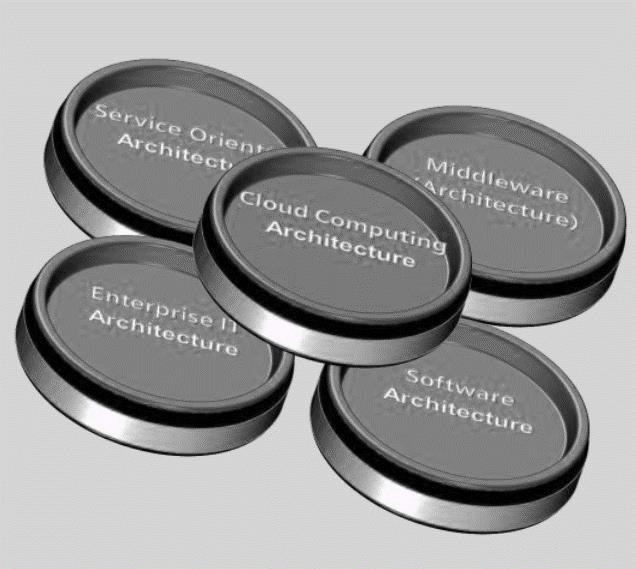
\includegraphics[scale=0.45]{fi1}
\caption{معماری محاسبات ابری در مجموعه سیستم‌های کامپیوتری
\cite{9}}\label{fig1}
\end{figure}
اما معماری کل محاسبات ابری ازلحاظ پیاده‌سازی را می‌توان در شکل
\ref{fig4} 
مشاهده نمود که به شرح زیر آن‌ها را توضیح خواهیم داد.
\begin{figure}
\centering
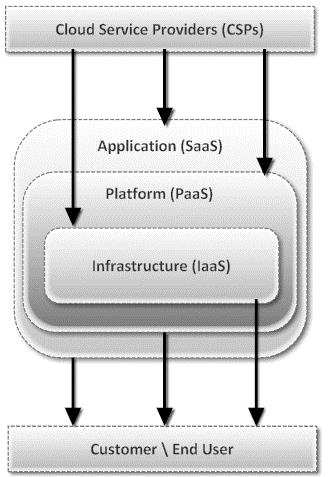
\includegraphics[scale=0.6]{fi2}
\caption{معماری ساختاری محاسبات ابری}\label{fig2}
\end{figure}
\subsection{فراهم‌کننده سرویس ابر}
فراهم‌کننده سرویس کسانی هستند که بستری برای استفاده از منابع موجود فراهم می‌کنند. سرویس‌دهندگان می‌توانند یک یا چند سرویس که در میانه شکل 
\ref{fig4}
نشان داده‌شده را فراهم کند؛ بنابراین می‌تواند سه دسته سرویس‌دهندگان نرم‌افزار، سرویس‌دهندگان بستر و سرویس‌دهندگان زیرساخت را معرفی نمود.
\subsection{انواع ارائه خدمت}
 در محیط محاسبات ابری عموماً سه خدمت عمده را به‌عنوان ساختار خدمات‌رسانی به‌صورت اولویت‌بندی شده ارائه می‌دهد؛ که به ترتیب ارائه نرم‌افزار به‌عنوان خدمت، ارائه بستر به‌عنوان خدمت و ارائه زیرساخت به‌عنوان خدمت نام دارند. در ابتدای این زنجیره نیز فراهم‌کنندگان قرار دارند و در انتها نیز کاربران می‌باشند.  

ارائه نرم‌افزار به‌عنوان خدمت در بالاترین و ساده‌ترین لایه محاسبات ابری مجموعه نرم‌افزارها به‌عنوان یک خدمت ارائه می‌گردد. تمام نرم‌افزارهای موجود را می‌تواند در این بخش ارائه نمود. پایگاه داده نیز می‌تواند در این بخش ارائه گردد. یکی از اولین ساده‌ترین نرم‌افزارها خدمات ایمیل می‌باشد که می‌توانید در آن‌ها پیام‌های خود را نگهداری و مدیریت کنید؛ اما امروزه برنامه‌هایی همچون مدیریت ارتباط با مشتری، مدیریت منابع سازمانی، مدیریت زنجیره چرخه و... نیز در این لایه ارائه می‌گردند
\cite{13}.
\subsection{کاربران محیط محاسبات ابری}
 کاربران این محیط را می‌تواند به دودسته تقسیم کرد: یکی استفاده‌کنندگان خدمت‌ها که تنها برای استفاده از خدمات درخواست می‌دهند و از آن‌ها استفاده می‌کنند و بر اساس مصرف خود هزینه پرداخت می‌کنند. کاربران دیگر محیط محاسبات ابری اعضای آن می‌باشند که می‌توانند در تهیه خدمات همکاری کنند.
\section{امنیت در محیط محاسبات ابری}
با توجه به روند روبه‌پیشرفت و توسعه استفاده از محاسبات ابری بسیاری از شرکت‌ها همچون 
\lr{EBay}، 
\lr{Microsoft}، 
\lr{Google}، 
\lr{Amazon}
 و ... با صرف میلیاردها دلار به خدمات‌دهی به مشتریان و کاربران خود در این زمینه پرداخته‌اند. با توجه به این سرمایه‌گذاری‌ها مطمئناً ایجاد امنیت برای اطلاعات مهم کاربران بسیار مهم می‌باشد. دو بخش بسیار مهم در محیط محاسبات ابری وجود دارد که می‌بایست ازلحاظ امنیتی موردتوجه قرار گیرند. یکی آسیب‌های ماشین‌های مجازی و دیگری جامعیت پیام‌ها می‌باشد.
 
برای ارائه هر خدمتی می‌بایست یک ماشین مجازی به کاربر ارائه گردد تا در محیط کاملاً کنترل‌شده‌ای بتواند از خدمات استفاده نماید. این باعث می‌شود تا هم کاربر در محیط خود احساس امنیت کند و از در امان بودن اطلاعات خود مطمئن باشد؛ و هم اینکه کاربر نتواند به محیط‌های غیرمجاز دسترسی داشته باشد و یا اینکه از محتویات سرور باخبر گردد؛ بنابراین ایجاد امنیت در این محیط بسیار مهم می‌باشد تا از سوءاستفاده دیگران و خرابکاری و یا دزدی اطلاعات و دیگر خطرات جلوگیری شود.

 نکته دوم و مهم برای حفظ امنیت، راه‌های ارتباطی تبادل اطلاعات بین ماشین‌های مجازی با یکدیگر و یا با سرور و هرگونه محیط دیگر می‌باشد؛ تا از نشت اطلاعات و یا سرقت اطلاعات شخصی کاربران جلوگیری شود؛ بنابراین می‌بایست در ارسال اطلاعات از روش‌های مختلفی برای جلوگیری از دزدی استفاده شود. در این راستا از روش‌هایی همچون رمزنگاری اطلاعات، استفاده از پروتکل‌های امن و نشانه‌گذاری پیام‌ها و یا تأیید صحت کاربران استفاده می‌شود.
 
هرچند امروزه گره‌های ابر بسیار موردتوجه مردم قرارگرفته‌اند اما بااین‌حال یکی از چالش‌های عمده‌ای که محاسبات ابری با آن روبرو است، چگونگی حفاظت از داده‌ها و برقراری امنیت فرآیندهای کاربران است، امنیتی که در محیط ابر فراهم می‌شود، برای سازمان‌ها و افراد بسیار حائز اهمیت است، چراکه برخی سازمان‌ها انتقال برنامه‌های کاربردی مهم و داده‌های حساس خود را به یک محیط ابر عمومی، یک ریسک بزرگ تلقی می‌کنند، بنابراین برای کاهش این نگرانی‌ها، یک ارائه‌دهنده ابر باید این اطمینان را ایجاد کند که مشتریان می‌توانند امنیت و کنترل حریم خصوصی خود را روی برنامه‌های کاربردی حفظ کنند، پس ارائه‌دهندگان ابر برای متقاعد کردن مشتریان خود در مورد مسائل امنیتی بایستی اقداماتی را انجام دهند، ازجمله می‌توان به " موافقت‌نامه سطح سرویس اشاره نمود. این موافقت‌نامه سندی است که ارتباط بین ارائه‌دهنده و دریافت‌کننده را مشخص می‌کند و در حقیقت یک توافق حقوقی بین ارائه‌دهنده سرویس و مشتری است.

مواردی که در خصوص جلب رضایت و اطمینان مشتری در موافقت‌نامه مطرح می‌شود، به شرح زیر می‌باشد.
\begin{itemize}
\item[$\bullet$]
شناسایی و تعریف نیازهای مشتری
\item[$\bullet$]
ساده‌سازی مسائل پیچیده
\item[$\bullet$]
کاهش زمینه‌های تعارض بین کاربران تشویق به گفت‌وگو در مورد برخوردها و اختلافات
\item[$\bullet$]
حذف انتظارات غیرواقعی
\item[$\bullet$]
ارائه چارچوبی برای درک راحت
\end{itemize}	 
همان‌طور که در جدول 
\ref{tab3} 
نشان داده‌شده است، برای پیاده‌سازی رویه و کنترل محاسبات ابری، اهمیت "امنیت" در حوزه‌های ریسک‌پذیر و بحرانی، برابر 
$7.91$ 
درصد است. در
\cite{14} 
نشان داده‌شده است که محیط مجازی ابرها به‌اندازه کافی ایمن و قابل‌اعتماد هستند.
\begin{table}[h!]
\caption{حوزه‌های ریسک‌پذیر و بحرانی در مجازی‌سازی و محاسبات ابری}
\label{tab1}
\begin{center}
\renewcommand{\arraystretch}{2}
\rowcolors{1}{white}{Gray!30}
\scalebox{0.88}{
\begin{tabular}{cccc}
\hline
درصد عدم
($\%$) &
درصد اهمیت
($\%$) &
درصد بحرانی بودن
($\%$) &
حوزه ریسک\/پذیر
\\
\hline
$0$ & $8.3$ & $91.7$ &
امنیت \\
\hline
$0$ & $58.3$ & $41.7$ &
مدیریت عملیات \\
\hline
$8.3$ & $50$ & $41.7$ &
 مدیریت تغییرات \\
\hline
$0$ & $33.3$ & $66.7$ &
حوادث و سوانح\\
\hline
$16.7$ & $41.7$ & $41.7$ &
  مدیریت سطح سرویس \\
\hline
$41.7$ & $50$ & $8.3$ &
مدیریت واسط\\
\hline
$25$ & $41.7$ & $33.3$ &
  آیین‌نامه و قوانین \\
\hline
\end{tabular}}
\end{center}
\end{table}
\subsection{تهدیدات امنیتی محیط محاسبات ابری}
با توجه به تحت اینترنت بودن محیط محاسبات ابری می‌تواند گستره بزرگی از حملات را برای آن در نظر گرفت به‌گونه‌ای که می‌تواند گفت تمامی حملات موجود در گونه‌های دیگر شبکه‌ها را در این محیط پیدا خواهیم نمود. در زیر برخی از این حملات را شرح خواهیم داد.
\subsubsection{حمله اخلال در خدمت‌رسانی}
یکی از رایج‌ترین حملات در این محیط حمله اخلال و یا انکار خدمت است که باعث مختل شدن سرویس‌دهنده می‌شود. حمله‌کننده در زمان مناسبی شروع به ارسال مداوم و سریع درخواست به سرویس‌دهنده می‌کند. در این حمله سیل‌آسا اگر تعداد درخواست‌کننده‌ها و درخواست‌های آن بیش‌ازاندازه باشد باعث می‌شود تا میزان پردازش سرویس‌دهنده بالا برود و باعث اخلال در کار آن می‌گردید و می‌تواند باعث هنگ کردن پردازشگر و یا پر شدن حافظه آن و یا گم‌شدن درخواست‌ها و غیره گردد.
\subsubsection{حمله شنود اطلاعات}
اگر لایه امنیتی 
\lr{SSL} 
به‌خوبی استفاده نشود حمله شنود اطلاعات انجام می‌پذیرد. در این حمله شخصی می‌تواند در بین افراد قرار گیرد و به شنود بپردازد و درنتیجه اطلاعات افراد را به سرقت ببرد؛ بنابراین می‌بایست لایه‌های امنیتی را به‌خوبی تنظیم نمود تا ازاین‌گونه حملات جلوگیری شود.
\subsubsection{دزدی اطلاعات شبکه}
اگر داده‌ها به‌خوبی رمزنگاری نشوند و از آن‌ها محافظت نگردد به‌راحتی به‌وسیله متهاجمان موردحمله و دستبرد قرار می‌گیرند. در این حمله مهاجم به کپی‌برداری از اطلاعات تبادل شده و یا نفوذ به فضای نگهداری اطلاعات به سرقت آن‌ها می‌پردازد.
\subsubsection{پویش درگاه}
گاهی مهاجمان به شنود و پویش درگاه‌های سیستم می‌پردازند تا از طریق آن‌ها در سیستم کاربران نفوذ کنند؛ مثل درگاه‌های عمومی همچون درگاه 
$80$
یا 
$8080$ 
همواره باز هستند و از طریق آن‌ها می‌توان به نفوذ پرداخت. برای نمونه مهاجم می‌تواند از راه این درگاه‌ها به نشر وب‌سرویس در سیستم کاربران بپردازد و در زمان مناسب آن‌ها را اجرا نماید و به تخریب و یا دزدی اطلاعات دست بزند.
\subsubsection{حمله دستورات 
\lr{SQL}}
یعنی اینکه درجاهایی که مثل نام کاربری و رمز عبور خواسته می‌شود به 
\lr{SQL} 
تزریق دستورات راحتی یک دستور پایگاه داده را قرارداد تا در زمان اجرا اطلاعات موردنیاز را از پایگاه داده واکشی نمود. این‌یکی از ساده‌ترین راه‌های نفوذ در شبکه می‌باشد که با انجام چند عمل پیشگیرانه می‌توان آن را برطرف نمود.
\subsubsection{تزریق بدافزار به ابر}
همان‌طور که در بخش قبل گفته شد ماشین‌های مجازی از مهم‌ترین بخشه‌ای ابر می‌باشد که همواره می‌تواند موردحمله قرار گیرد. در این راستا مهاجم می‌تواند بدافزار موردنظر خود را در ماشین مجازی تزریق نماید و پس‌ازآن به اجرای آن دست بزند. آنگاه می‌تواند از طریق آن به ماشین مجازی و یا سخت‌افزار و حتی سرورها صدمه‌های شدید وارد نماید.
\subsubsection{نفوذ از طریق رابط کاربری ضعیف}
 اگر رابطی که برای ایجاد ارتباط با برنامه‌ها در سرور و ماشین‌های مجازی طراحی کردیم ازلحاظ، امنیتی ضعیف و دارای رخنه‌های امنیتی باشند می‌تواند با استفاده از آن‌ها در سیستم نفوذ نمود. در اینجا نیز می‌تواند اطلاعات موردنیاز خود را از نشست‌ها و کوکی‌ها دریافت نمود و یا حتی فایل‌های مخرب را در آن‌ها قرارداد.
\subsubsection{خودی‌های مخرب}
کاربران ابر نیز می‌توانند خود باعث خرابی شوند. گاه این خرابکاری آگاهانه و گاهی ناخودآگاه می‌باشد؛ مثل با سهل‌انگاری توسط کاربران زمینه برای نفوذ و یا سرقت اطلاعات برای مهاجمان فراهم می‌شود. کاربران باید در این زمینه آموزش‌های مناسب را فراگیرند تا از سرقت اطلاعات جلوگیری شود.
\subsubsection{حمله ربات‌ها}
 یکی از مهم‌ترین و رایج‌ترین حملات در محیط محاسبات ابری که بیشتر مربوط به ماشین‌ها مجازی می‌باشد، حمله ربات‌ها می‌باشد. در این نوع از حمله می‌تواند کنترل یک یا چند سیستم کاربر را به‌عنوان سیستم قربانی به دست گرفت و از طریق آن‌ها به انجام حمله پرداخت. به سیستم‌های قربانی در اصطلاح زامبی گفته می‌شود چراکه دیگر کنترل آن‌ها در دست کاربر نیست.
 \section{سیستم‌های تشخیص نفوذ}
 تشخیص نفوذ عبارت است از تحلیل بی‌درنگ داده‌های شبکه به‌منظور تشخیص و ثبت و اخطار به هنگام بروز حملات و یا اقدامات مخرب امنیتی. در عمل انواع مختلفی از روش‌های تشخیص حمله وجود دارد که با توجه با انواع مختلف اقدامات درون شبکه قادر هستند اقدامات مخرب و نفوذی را کشف کنند. در عین این دستگاه‌ها از بخش‌های مختلفی تشکیل‌شده‌اند و به طرق مختلفی این اجزا می‌توانند در کنار هم قرار گیرند و عملکرد خاصی را ایجاد کنند. در این بخش به ارائه چارچوب کلی در مورد امنیت شبکه و سیستم‌های کامپیوتری می‌پردازیم. ابتدا انواع حملات و تهدیدهای موجود در شبکه‌های کامپیوتری را طبقه‌بندی می‌کنیم. سپس به طبقه‌بندی سیستم‌های تشخیص نفوذ از حیث ساختار می‌پردازیم. درنهایت هم در مورد تکنولوژی‌های تشخیص نفوذ و کارکردهای مختلف این ابزارها در مدیریت و حفظ امنیت و نظارت بر شبکه‌های کامپیوتری بحث می‌کنیم.
 \subsection{انواع حملات شبکه‌ای با توجه به حمله‌کننده}
  حملات شبکه‌ای را می‌تواند با توجه به حمله‌کننده به چهار گروه تقسیم کرد:
  \\[0.5cm]
 حملات انجام‌شده توسط کاربر مورد اعتماد داخلی: این حمله یکی از مهم‌ترین و خطرناک‌ترین نوع حملات است، چون ازیک‌طرف کاربر به منابع مختلف شبکه دسترسی دارد و از طرف دیگر سیاست‌های امنیتی معمولاً محدودیت‌های کافی درباره این کاربران اعمال نمی‌کنند.
 \\[0.5cm]
 حملات انجام‌شده توسط افراد غیر معتمد خارجی: این معمول‌ترین نوع حمله است که یک کاربر خارجی که مورد اعتماد نیست شبکه را موردحمله قرار می‌دهد. این افراد معمولاً سخت‌ترین راه را پیش رودارند زیرا بیشتر سیاست‌های امنیتی درباره این افراد تنظیم‌شده‌اند.
 \\[0.5cm]
حملات انجام‌شده توسط مهاجم‌های بی‌تجربه: بسیاری از ابزارهای حمله و نفوذ بر روی اینترنت وجود دارند. درواقع بسیاری از افراد می‌توانند بدون تجربه خاصی و تنها با استفاده از ابزارهای آماده برای شبکه ایجاد مشکل کنند. حملات انجام‌شده توسط کاربران مجرب: مهاجم‌های باتجربه و حرفه‌ای در نوشتن انواع کدهای خطرناک متبحرند. آن‌ها از شبکه و پروتکل‌های آن و همچنین از انواع سیستم‌های عامل آگاهی کامل دارند. معمولاً این افراد ابزارهایی تولید می‌کنند که توسط گروه اول به کار گرفته می‌شدند. آن‌ها معمولاً پیش از هر مرحله، آگاهی کافی درباره هدف خود و آسیب‌پذیری‌های آن کسب می‌کنند.
\section{انواع سیستم‌های تشخیص نفوذ}
 سیستم‌های تشخیص نفوذ با توجه به نحوه کاربری و محل نصب و میزبان یا شبکه‌ای که از آن محافظت می‌کنند، می‌تواند مبتنی بر میزبان، شبکه یا به‌صورت توزیع‌شده عمل کنند.
 \subsection{سیستم‌های تشخیص نفوذ مبتنی بر میزبان}
 این دستگاه‌ها از یک میزبان در مقابل عملیات نفوذی و مخرب محافظت می‌کند. این سامانه محافظتی بر روی سیستم اجرا می‌شود و تمام فعالیت‌ها و فرآیندهای درون سیستم را کنترل می‌کند. 
 \lr{HIDS} 
 می‌تواند واسط شبکه‌ای را نیز پویش دهد و بر دسترسی‌هایی که از خارج به سیستم می‌شود، نظارت کند. این نوع از سیستم تشخیص نفوذ بر روی خود سیستم اجرا می‌شود و از منابع خود سیستم مثل حافظه و پردازنده و... استفاده می‌کند. 
 \lr{HIDS} 
 عمل کنترل دسترسی‌ها را انجام می دهدو بررسی می‌کند که چه پردازه‌هایی از چه منابعی استفاده می‌کنند. برای مثال دسترسی یک برنامه با عنوان پردازشگر متن به اطلاعات حساس سیستم مثل رمز محل ذخیره عبور، یک اقدام مشکوک است. همچنین به بررسی مداوم وضعیت سیستم می‌پردازد و منابع سخت‌افزاری و اطلاعاتی سیستم را در مورد دسترسی و ویرایش توسط عوامل مشکوک بررسی می‌کند. امروزه بسیاری از برنامه‌های امنیتی تحت عنوان ضدویروس برای حفظ امنیت سیستم کامپیوتری به کار می‌روند. این دستگاه‌ها بیشتر وقت خود را صرف کنترل دسترسی پردازه‌ها می‌کنند. این‌که هرکدام از پردازه‌ها به چه منابعی می‌تواند و یا نمی‌توانند دسترسی داشته باشد. یک 
 \lr{HIDS} 
 می‌تواند سیاست‌های امنیتی خاص را بر روی سیستم اعمال کند و در مقابل حملات منجر به اشباع شدن منابع سیستم از آن حفاظت کند.
 
 در بسیاری از موارد حمله‌کننده عملیات نفوذ را در چند مرحله صورت می‌دهند. مهاجم‌ها در بیشتر موارد هدف چنین مهاجم‌هایی تصاحب منابع سیستم است، به نحوی نرم‌افزار خاصی بر روی سیستم نصب کنند و یا تغییر موردنظر خود را در اطلاعات سیستم ایجاد کنند. ازنظر تئوری تمام اقدامات نفوذی به این نحو امکان‌پذیر است بسیاری از این اقدامات توسط سیستم‌های تشخیص نفوذ تحت شبکه
 \lr{(NIDS)} 
 کشف می‌شوند. سیستم‌های 
 \lr{HIDS} 
 در تکمیل کار 
 \lr{NIDS} 
 سعی در کشف نفوذهای کشف نشده توسط 
 \lr{NIDS} 
 دارند. به لحاظ تکنیکی راه‌حل‌های نرم‌افزاری برای ایجاد همکاری بین این دو سیستم امکان‌پذیر است.
 عمل نظارت معمولاً به این صورت انجام می‌شود که از تمام اشیاء سیستمی مهم به‌طورمعمول اشیاء سیستم فایل) یک نمونه درهم‌سازی شده تولید می‌شود و در یک پایگاه داده مطمئن ذخیره می‌شود. به‌مرورزمان با بررسی آن می‌تواند فهمید که کدام‌یک از اشیاء سیستم می‌تواند دسترسی به نقاط حساس سیستم را کنترل 
 \lr{HIDS} 
 دچار تغییر ناخواسته شده‌اند. به‌عنوان‌مثال قسمت‌های خاصی از فضای حافظه یا جدول فراخوانی‌های سیستمی مربوط به سیستم‌عامل.
\subsection{سیستم‌های تشخیص نفوذ مبتنی بر شبکه}
 این سیستم ها در بستر شبکه فعالیت می‌کنند و با پویش ترافیک شبکه و تحلیل آن در تمام لایه‌های مختلف شبکه، به دنبال کشف نشانه‌های اقدامات نفوذی و یا حملات هستند. انواع حملاتی که در سطح شبکه می‌توانند وجود داشته باشند شامل حملات 
 \lr{DoS}، 
 حملات پویش درگاه هستند. معمولاً این سیستم ها از چندین حسگر نقاط مختلف برای دریافت ترافیک شبکه برخوردارند. ویژگی‌های دریافت شده از این ترافیک به پایگاه مرکزی تحلیل فرستاده می‌شود تا بر اساس روش‌های مختلف تشخیص نفوذ، اقدامات نفوذی آشکار شوند.
 \section{اجزای تشکیل‌دهنده سیستم‌های تشخیص نفوذ مبتنی بر شبکه}
 اجزای اصلی این دستگاه‌ها عبارت‌اند از حسگر، سرور مدیریت و تحلیل، سرور پایگاه داده، چندین واسط کاربری و سرورهای پایگاه داده. حسگر جزئی است که ترافیک شبکه مربوط به یک یا چند بخش را پویش می‌کند. واسط شبکه‌ای حسگرها طوری پیکربندی‌شده‌اند که تمام بسته‌های دریافتی را بدون در نظر گرفتن آدرس مقصد دریافت می‌کند. تمام حسگرها دریکی از این دو نوع هستند:
 \begin{itemize}
 \item[$\bullet$]
 نوع مبتنی بر سخت‌افزار: این نوع حسگر شامل سخت‌افزار خاص‌منظوره طراحی‌شده که به همراه نرم‌افزار اجرا شوند بر روی آن است. سخت‌افزار برای استفاده جهت کاربرد حسگر بهینه‌سازی شده است و کارت‌های واسط شبکه‌ای خاصی بر روی آن‌ها قرارگرفته که تمام ترافیک عبوری را دریافت می‌کند. این افزارها معمولاً شامل سیستم‌عاملی هستند که به‌صورت مستقیم توسط مدیر سیستم مورد دسترسی نیست، ولی واسط نرم‌افزاری مناسب امکان ارتباط با کاربر و بخش‌های دیگر سیستم تشخیص نفوذ را فراهم می‌کند.
 \item[$\bullet$]
 نوع مبتنی بر نرم‌افزار: ابزار تشخیص نفوذ به‌عنوان یک نرم‌افزار عرضه می‌شود. در این حالت ممکن است نرم‌افزار به همراه سیستم‌عامل مربوط به آن ارائه شود یا آنکه نرم‌افزار قابل‌نصب بر روی سیستم‌عامل‌های همه‌منظوره باشد. بسیاری از ابزارهای تشخیص نفوذ در این حالت قابل پیکربندی هستند.
 \end{itemize}
\subsection{سیستم‌های توزیع‌شده}	
امروزه با روند افزایش پهنای باند شبکه‌ها و نیاز به پویش بی‌وقفه این داده‌ها، سیستمهای تشخیص نفوذ تحت شبکه هم باید همگام با آن‌ها توسعه پیدا کنند. امروزه روش‌های معماری‌های متمرکز مبتنی بر شبکه، جوابگوی شبکه‌های امروزی نیست. این روش‌ها برای تشخیص حملات چندمرحله‌ای و نگهداری وضعیت انواع ارتباطات و نیز مراودات پروتکلی در جریان، به خاطر وجود یک نقطه سرویس‌دهی، سیستم دچار کوبیدگی%
\LTRfootnote{Thrashing}
  و افت گذردهی می‌شود. الگوریتم‌های تشخیص نفوذ مبتنی بر یک سری قوانین هستند که به‌سرعت در حال بزرگ شدن هستند. ایجاد 
\lr{IDS}های 
توزیع‌شده نیاز به تمهیداتی برای معماری شبکه‌ای، نرم‌افزار مناسب برای عملکرد توزیع‌شده و تقسیم ترافیک شبکه بین بخش‌های موازی دارد.
\begin{figure}
\centering
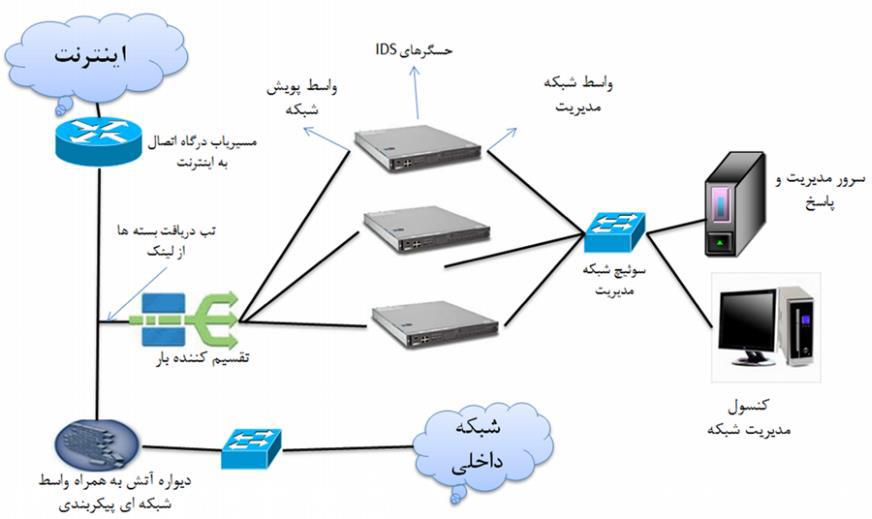
\includegraphics[scale=0.6]{fi3}
\caption{معماری 
\lr{IDS}های 
توزیع‌شده با استفاده از حسگرهای بی‌اثر و با امکان توزیع بار}\label{fig3}
\end{figure}
  برای عملکرد 
 \lr{IDS}های 
 توزیع‌شده، دو نوع تکنیک مطرح وجود دارد: تقسیم ترافیک و متعادل کردن بار. روش‌های مبتنی بر تقسیم ترافیک بیشتر بر اساس جریان‌های دادهای و سیاست‌های امنیتی و ساختار 
 \lr{IDS} 
 و با این هدف‌ها کار می‌کنند:
 
بسته‌های مربوط به هرکدام از حمله‌کننده‌های احتمالی به یک حسگر وارد شود.

 بر اساس سرعت و پهنای باند شبکه عملکرد و بهره‌وری حفظ شود.
 
 تطابق‌پذیری سیستم در شرایطی با ترافیک‌های مختلف.
 
روش‌های مبتنی بر تعادل بار در هر زمان مقدار بار مناسبی برای هرکدام از حسگرها در نظر می‌گیرد به‌نحوی‌که از ظرفیت سیستم به نحو بهینه استفاده شود. تعادل بار می‌تواند به دو صورت برآورده شود:

استفاده از تسهیم کننده بار: این ابزار در ورودی شبکه قرار می‌گیرد و کل ترافیک شبکه باید از آن عبور نماید. به همین دلیل بایستی ابزار مورداستفاده توانمندی بالایی داشته باشد تا به گلوگاه عبور ترافیک تبدیل نشود.

 هرکدام از حسگرها با استفاده از چندین الگوریتم تسهیم بار و انجام محاسبات خاص، حسگرهایی را که دچار بار بیش‌ازحد شده‌اند را تعیین کرده و با انجام تنظیم‌های خاص، باعث می‌شود که بار ورودی به آن‌ها کاهش یابد. این عملیات با روش‌های مختلفی می‌تواند صورت پذیرد. ازجمله فیلتر کردن زودرس که بعضی از بسته‌ها در خود تسهیم کننده بار پردازش می‌شدند. روش دیگر استفاده از یک گره مرکزی است که از دیگر گره‌ها پیغام‌هایی را دریافت می‌کند و بار زیاد بر روی هرکدام از حسگرها و یا بروز حملات توزیع‌شده در شبکه یا حملات چندمرحله‌ای را متوجه می‌شود. بعدازاین مرحله این گره با ارسال فرمان‌های کنترلی باعث می‌شود که جریان بسته‌ها در حسگرها به نحو پویا تنظیم شود. این الگوریتم‌ها پیچیدگی بالایی دارند ولی در صورت پیاده‌سازی موفق، بهره‌وری قابل‌توجهی دارند.
 
موازی‌سازی در سطح بسته‌ها: در این حالت یک تسهیم کننده بار باسیاست گردشی، بسته‌ها رابین حسگرها تقسیم می‌کند. در این صورت تعادل بار به نحو مناسبی صورت می‌گیرد. بااین‌حال برای ایجاد حالت مندی و حفظ اطلاعات جریان‌های مختلف و مراودات پروتکلی مختلف و همین‌طور داشتن اطلاعات کامل از هر ارتباط، نیاز به عنصری تحت عنوان تحلیل‌گر ارتباطات هستیم. این عنصر تمام داده‌های موردنیاز خود را از طریق پیش پردازنده‌ها به دست می‌آورد. در ساختار چنین سیستمی باید هریک از حسگرها با این تحلیلگر ارتباطات، ارتباط مناسب و امنی داشته باشند. همچنین در پیاده‌سازی آن باید دقت بسیاری شود، چون به‌سادگی می‌تواند به گلوگاه بهره‌وری تبدیل شود.

موازی‌سازی در سطح ارتباطات و مراودات پروتکلی: در این روش در تسهیم کننده بار، توزیع بسته‌ها به روشی صورت می‌گیرد تا بسته‌های مربوط به هرکدام از ارتباطات به یک حس گر وارد شوند. در این حالت وجود جدول‌ها و اطلاعات مربوط به هرکدام از جریان‌ها در هر یک از حسگرها ضروری است. در این ساختار باید توجه شود که باید برای تشخیص حملات چندمرحله‌ای و حملات مربوط به چندین ارتباط، نیاز به عنصری تحت عنوان تحلیلگر شبکه‌داریم. این عنصر باید توانایی تحلیل رویدادهای مربوط به جریان‌های مجزا و ایجاد ارتباط بین این رویدادها را داشته باشد. این روش موازی‌سازی هیچ تضمینی در مورد تقسیم عادلانه بار ارائه نمی‌دهد.

موازی‌سازی در سطح قوانين: در این روش قوانین موجود در 
\lr{IDS} 
بین حسگرهای مختلف تقسیم می‌شود. عنصری در ابتدای مسیر تحت عنوان 
\lr{Traffic Duplicator} 
یک کپی از ترافیک را برای هرکدام از بسته‌ها می‌فرستد. به‌این‌ترتیب هرکدام از حسگرها مسئول اعمال تعداد محدودی از قوانین بر روی بسته‌ها می‌باشد. در صورت تقسیم مناسب قوانین بین حسگرها و اعمال قوانین از یک کلاس و دسته به یک حسگر خاص، عمل تشخیص به بهترین نحو صورت گرفته و تعادل بار صورت می‌گیرد. بااین‌حال، هرکدام از حسگرها باید جداگانه عملیات پیش‌پردازش و حذف بسته‌های زائد را انجام دهد که اتلاف منابع را نسبت به روش‌های دیگر در پی دارد.
\section{انواع روش‌های تشخیص حمله}
ابزارهای تشخیص نفوذ از روش‌های مختلفی برای تشخیص انواع مختلف حملات استفاده می‌کنند.  

این روش‌ها را می‌تواند در سه کلاس مبتنی بر امضا، تشخیص ناهنجاری و مبتنی بر تحلیل حالت پروتکل ارتباطی دسته‌بندی کرد.
\subsection{روش‌های مبتنی بر امضا}	
امضا یا ویژگی عبارت است از الگوی مربوط به یک عملیات مشخص. وجود یک فرمان اجرایی دربسته که برای افزایش سطح دسترسی به سیستم موردنظر ممکن است مورداستفاده قرار گیرد؛ مانند فرمان دسترسی 
\lr{root} 
روش تشخیص مبتنی بر امضا عبارت است از مقایسه الگوی رفتارهای در جریان در شبکه با نمونه‌های مشاهده‌شده به‌منظور مشخص کردن امکان بروز حملات. این روش تشخیص حملات در برابر طیف حملات شایع و شناخته‌شده بسیار مؤثر و نتیجه‌بخش است. لکن با توجه به انواع مختلف حملات و الگوهای رفتاری متنوعی که می‌تواند توسط مهاجمین به کار گرفته شود، بازدهی این روش محدود می‌شود. به‌عنوان نمونه در مثال ایمیل‌هایی که ضمیمه فایل اجرایی داشتند، چنانچه نام فایل اجرایی ضمیمه به 
"\lr{FREEPics.exe}" 
تغییر یابد، این روش قادر به تشخیص این نوع نفوذ نخواهد بود.

 روش تشخیص مبتنی بر امضا ساده‌ترین روش تشخیص حملات به شبکه‌های کامپیوتری می- باشد، زیرا در این روش فقط فعالیت در جریان فعلی موردبررسی قرار می‌گیرد؛ مانند فرآیند آخرین بسته دریافتی یا گزارش آخرین فعالیت صورت گرفته. در این عملیات با استفاده از روش‌های مقایسه رشته‌های حرفی، مقایسه‌ای با فهرستی از الگوهای موجود صورت می‌گیرد. این روش کار آیی اندکی در مقابل ارتباطات پیچیده‌تری که طی چند مرحله صورت می‌گیرند و در هر مرحله در وضعیت خاصی به سرمی برند، دارد. این روش‌ها قادر نیستند درخواست ارسال‌شده را با پاسخ مربوط به آن کنار هم ارسالی را با پاسخ مربوط به 
 \lr{HTTP} 
 قرار دهند. برای مثال قادر نیستند در یک ارتباط وب درخواست آن باهم در نظر بگیرند. این روش‌ها همچنین قادر نیستند درخواست‌های قبلی یک کاربر را با درخواست‌های فعلی او باهم در نظر بگیرند. حفظ نکردن وضعیت، محدودیت‌های جدی به همراه دارد. این روش‌ها در مقابل حملاتی که از چند مرحله تشکیل‌شده‌اند و مبتنی بر یک سری رخداد پیاپی هستند ناکام‌اند، مگر اینکه هرکدام از مراحل شامل نشانه و یا الگوی مشخصی، دال بر بروز حمله داشته باشند.
 \subsection{روش‌های تشخیص حمله مبتنی بر ناهنجاری} 
روش‌های مبتنی بر تشخیص ناهنجاری عبارت است از مقایسه شرایط عادی سیستم با شرایط مشاهده‌شده، به‌منظور تشخیص تفاوت‌های جدی که معمولاً در صورت بروز حملات رخ می‌دهد. دستگاه‌هایی که بر اساس این روش‌ها عمل می‌کنند، دارای سابقه‌های مستندی هستند که نمود وضعیت اجزای مختلف سیستم در وضعیت عادی است. وضعیت ارتباطات، تعداد مشترکین، وضعیت رفتاری و درخواست‌های معمول مشترکین و نیز مناسبات نرم‌افزاری و سخت‌افزاری در جریان از آن جمله‌اند. این سابقه‌ها با بررسی و ثبت عملکرد کاربران و وضعیت سیستم در یک دوره زمانی مشخص به دست می‌آیند. برای مثال این مستندات ممکن است نشان دهند که استفاده از وب در حدود 
$40$
درصد فعالیت کاربران شبکه و نیز پهنای باند در دسترس را نشان می‌دهد. ابزار تشخیص نفوذ بر اساس روش‌های ایستایی ویژگی‌های وضعیت فعلی را اندازه‌گیری می‌کند و با حدود آستانه‌ای که در سابقه سیستم ثبت‌شده است مقایسه می‌کند. برای مثال ممکن است نسبت ترافیک وب از حد بالای آستانه بیشتر شود. همچنین پارامترهای دیگری می‌توانند موردبررسی قرار بگیرند. از آن جمله می‌تواند تعداد ایمیل‌های ارسالی و یا دریافتی، تعداد دفعات تلاش برای واردکردن رمز و ورود به سیستم و یا درصد به‌کارگیری پردازنده در یک دوره زمانی اشاره کرد.  

به‌عنوان یک نمونه دیگر از به‌کارگیری این روش‌ها می‌توان به تشخیص حملات سرریز اشاره کرد. در حالت عادی بعد با توجه به مراحل دست دهی سه‌گانه 
\lr{TCP}، 
به‌طورمعمول باید تعداد بسته‌های درخواست ایجاد ارتباط با پرچم 
\lr{SYN} 
با بسته‌های پاسخ ارتباط 
\lr{TCP} 
که دارای پرچم‌های 
\lr{SYN} 
و 
\lr{Ack} 
هستند، برابر باشند. درصورتی‌که تعداد بسته‌های نوع نخست افزایش فرآیندهای نسبت به نوع دوم داشته باشد، این نشانه می‌تواند دلیلی بر بروز حملات 
\lr{DoS} 
باشد.  

مزیت عمده روش‌های مبتنی بر تشخیص ناهنجاری این است که می‌تواند با صرف کمترین هزینه، انواع مختلف و ناشناخته‌ای از حملات را که الگوی آن‌ها قبل مشاهده نشده را تشخیص دهد. برای مثال حملاتی که در آن‌ها پردازنده سرور مشغول می‌شود، یا آنکه تعداد زیادی ایمیل فرستاده می‌شود، یا تعداد زیادی ارتباط بی‌مورد برای مشغول نگه‌داشتن سرور به سمت آن ایجاد می‌شود، با این روش قابل‌تشخیص‌اند.

سابقه سیستم مورداستفاده در این دستگاه‌ها در یک‌فاز آموزش که ممکن است روزها و یا هفته‌ها ادامه داشته باشد، ثبت و بررسی می‌شود. این پرونده‌ها می‌توانند به‌صورت ثابت باشند، یا در طول زمان به‌صورت تطبیقی تغییر داده شوند. درروش اول اطلاعات ثابت باقی می‌مانند مگر آنکه به‌طور صریح از طرف مدیر سیستم، فاز آموزش ازسرگیری شود. به این دلیل که رفتارها و پارامترهای وضعیتی دستگاه‌ها دارای توزیعی نرمال هستند و در طول زمان تغییر می‌کنند. درروش پروفایل‌های تطبیقی مشکل کمتری به‌مرورزمان پیش می‌آید. لکن این امکان وجود دارد که حمله‌کننده با صرف زمان، به‌مرور و مرحله‌به‌مرحله تغییرات موردنظر را ایجاد کند و باگذشت زمان این رفتار برای سیستم تشخیص نفوذ تغییر رفتار عادی جلوه کند. از دیگر مشکلات سیستم‌های مبتنی بر ناهنجاری این است که ممکن است در فاز آموزش، سیستم حمله‌کننده وضعیت مطلوب خود را در سابقه سیستم ثبت کند. باید پذیرفت که رفتارهای این‌چنینی با احتمال زیاد در سابقه سیستم ثبت می‌شدند.

از دیگر مسائل مربوط به روش‌های تشخیص مبتنی بر ناهنجاری این است که به خاطر پیچیدگی و تنوع رفتارهای مختلفی که در یک شبکه ممکن هستند، اولاً ایجاد این سابقه به‌دقت زیادی نیاز دارد، ثانیه تشخیص دقیق علت بروز ناهنجاری ممکن نیست. ممکن است عملیات بروز رسانی سیستم که نیازمند انتقالات داده و ارتباطات زیادی است در فاز آموزش‌دیده نشود. به‌این‌ترتیب در زمان کار سیستم راه‌اندازی چنین تغییراتی به‌خودی‌خود موجب اخطارت بی‌مورد و غلط می‌شود. در حالاتی که سیستم اخطار تولید می‌کند، بررسی اینکه اخطار، دلیل درست و موجهی دارد دشوار است.

 از سوی دیگر تعیین نوع حمله و روزنه امنیتی آسیب‌پذیر در مقابل حمله، بر اساس پارامترهای اندازه‌گیری شده کاری دشوار است. بسیاری حملات ممکن است بدون نیاز به تغییرات اساسی در وضعیت سیستم، به نقاط ممنوعه آن واردشده و اطلاعات را تخریب یا سرقت کنند. لکن با توجه به اینکه تغییرات اساسی در وضعیت سیستم رخ نداده است، تشخیص این حملات بر اساس این روش‌ها دشوار و یا ناممکن است.
 \subsection{روش‌های مبتنی بر تحلیل حالت پروتکل ارتباطی} 
 این روش به فرآیندی گفته می‌شود که طی آن روند رخدادهایی که در جریان ارتباط‌های مختلف به وقوع می‌پیوندند، با نمونه‌های سلسله رخداد مربوط به پروتکل‌های مناسب و غیر مهاجم مقایسه می‌شدند تا درصورتی‌که مجموعه رخدادهای در جریان، ناشناس و یا مشکوک تشخیص داده شود، سیستم آن را تشخیص دهد. برخلاف روش مبتنی بر تشخیص ناهنجاری که بر سابقه رفتارهای شبکه خاص تکیه داشت، در اینجا پروفایل‌های موردبررسی مربوط به پروتکل‌های خوش‌تعریف، جامع و مشخصی است که کاملاً شناخته‌شده هستند و روند اجرای آن‌ها مشخص است و هرگونه تخطی از کاربرد درست آن‌ها می‌تواند یک رخداد مشکوک به تجاوز به شبکه باشد. کاربرد روش‌های مبتنی بر پروتکل به این معنی است که ابزار تشخیص نفوذ قادر به فهم و تشخیص و پیگیری روند اجرای پروتکل‌های لایه انتقال و کاربرد هست.
 
برای مثال در یک ارتباط 
\lr{FTP}
که در دو مد قابل انجام است، در مد کاربران غیرمجاز فقط اقداماتی از قبیل مشاهده لیست راهنما و واردکردن نام کاربری و شناسه عبور مجاز است. در این وضعیت ابزار تشخیص نفوذ می‌تواند زوج درخواست کاربر و پاسخ سرور را باهم مطابقت دهد و مشخص کند که آیا هرکدام از درخواست‌های کاربر برای وارد شدن به سیستم موفق بوده است یا نه. به‌محض اینکه شناسه کاربر تائید شد و کاربر به سیستم وارد شد، کاربر قادر به انجام اقدامات مختلف هست. صدور هر یک از فرامین مربوط به کاربران واردشده به سیستم از سوی کاربری که هنوز وارد سیستم نشده است می‌تواند مشکوک به یک فعالیت مخرب در جهت نفوذ به سیستم باشد.

 در روش تشخیص نفوذ مبتنی بر پروتکل امکان پیگیری روند ارسال فرمان‌ها از کاربران وجود دارد؛ به‌این‌ترتیب فرامین نامربوط قابل‌تعقیب‌اند. برای مثال صدور فرمان‌هایی خارج از روند پروتکل و یا ارسال پیغام‌های مربوط به یک‌فاز پروتکل به‌دفعات متعدد. این دستگاه‌ها همچنین قادرند بر اساس رده‌های کاربری مختلف و تعیین سطح دسترسی آن‌ها، فعالیت آن‌ها را پیگیری کنند. همچنین روند بررسی طول دستورات و آرگومان‌ها می‌تواند به‌صورت مجزا بر روی هرکدام از دستورات پروتکلی لایه کاربرد صورت گیرد. هرکدام از دستورات تعداد آرگومان‌های مشخص دارند که طول آن‌ها مشخص است. برای مثال دستوری می‌تواند 
 $2$ 
 آرگومان با حداکثر طول 
 $20$
 کاراکتر داشته باشد. درصورتی‌که تعداد آرگومان‌ها و یا طول آن‌ها مثلاً دستوری با طول از این حد تخطی کند، می‌تواند نشانه یک اقدام مشکوک باشد.
 
روش‌های مبتنی بر تحلیل پروتکل بر اساس مدل‌های پروتکلی استانداردی که توسط توسعه‌دهندگان نرم‌افزارهای شبکه معرفی می‌شدند و یا استانداردهای اینترنتی مشخص ثبت‌شده صورت می‌گیرد. در بسیاری از موارد جزئیات دقیق پروتکل به‌طور دقیق در مستندات مربوطه آورده نمی‌شود. در بسیاری از موارد، توسعه‌دهندگان نرم‌افزار با تخطی از مستندات پروتکل، در پیاده‌سازی‌های مختلف ویژگی‌های خاصی بر اساس نیاز به پیاده‌سازی پروتکل اضافه می‌شود. در بعضی موارد در مورد پروتکل‌هایی که کاربرد خصوصی دارند و در انحصار مالک هستند اطلاعات دقیقی در دسترس نیست. در تمام موارد ذکرشده، بعد از بروز رسانی پروتکل‌ها و یا معرفی پروتکل‌های جدید مدل پروتکلی ابزار تشخیص نفوذ باید بر اساس تغییرات صورت گرفته بروز رسانی شود. بااین‌حال مهم‌ترین ایراد روش‌های مبتنی بر پروتکل این است که این روش‌ها به منابع سخت‌افزاری و نرم‌افزاری زیادی نیاز دارند. پیچیدگی تحلیل پروتکل‌های متعدد و نگهداری وضعیت و پیگیری روند اجرای مربوط به هرکدام از مراودات پروتکلی در جریان، سربار زیادی را به سیستم تحمیل می‌کند. مشکل جدی دیگر این است که این روش‌ها برای تشخیص حملاتی که بر اساس الگوهای پروتکلی استاندارد عمل می‌کنند دچار مشکل هستند؛ مانند حملاتی که با ایجاد تعداد زیادی ارتباط پروتکلی صورت می‌گیرند و با مشغول کردن سرور و گرفتن منابع آن در وضعیت انتظار صورت می‌گیرند. حملات جلوگیری از سرویس گیری، گذشته از این‌ها در مواردی که ارتباط خدمتگزار و مشتری بر اساس پیاده‌سازی خاص پروتکل صورت گیرد یا آنکه پیغام‌ها رمز شده باشند، علاوه بر اینکه سیستم در تشخیص حملات واقعی ممکن است دچار اشتباه شود، ممکن است در بعضی موارد هشدارهای بی‌مورد تولید کند.
\chapter{ادبیات تحقیق}
 \section{مقدمه}
 تشخیص نفوذ عبارت است از تحلیل بی‌درنگ داده‌های شبکه به‌منظور تشخیص و ثبت و اخطار به هنگام بروز حملات و یا اقدامات مخرب امنیتی. در عمل انواع مختلفی از روش‌های تشخیص حمله وجود دارد که با توجه با انواع مختلف اقدامات درون شبکه قادر هستند اقدامات مخرب و نفوذی را کشف کنند. در عین این دستگاه‌ها از بخش‌های مختلفی تشکیل‌شده‌اند و به طرق مختلفی این اجزا می‌توانند در کنار هم قرار گیرند و عملکرد خاصی را ایجاد کنند. در این بخش به ارائه چارچوب کلی در مورد امنیت شبکه و سیستم‌های کامپیوتری می‌پردازیم. 
 
 در این فصل به بررسی تکنولوژی‌های تشخیص نفوذ و برخی از بهترین مطالعات انجام‌شده در این زمینه خواهیم پرداخت و هریک از آن‌ها را به همراه مزایا و معایب آن‌ها موردبررسی قرار می‌دهیم.
 \section{سیستم‌های تشخیص نفوذ و مدیریت ورودی چند سطحی در محاسبات ابری 
 \cite{29}}
 روش دیگری که برای محافظت از محیط ابری طراحی شد در این مقاله می‌باشد. در این مقاله حملات با توجه به میزان خسارت و همچنین سطح حملات آن‌ها در محیط ابری دسته‌بندی شدند بر این اساس برای هر حمله یک ریسک خطر تهیه و به آن‌ها داده شد و بر اساس آن روشی برای مقابله با آن در نظر گرفته‌شده است. در جدول 
 \ref{tab2}
 می‌توانید این دسته‌بندی و شماره‌های سطح داده‌شده به برخی حملات مهم را ببینید.
 \begin{table}[h!]
\caption{دسته‌بندی حملات با توجه به میزان خسارت}
\label{tab1}
\begin{center}
\renewcommand{\arraystretch}{2}
\rowcolors{1}{white}{Gray!30}
\scalebox{0.88}{
\begin{tabular}{|c|c|}
\hline
نوع ترافیک فعالیت ناهنجاری &	
میزان ریسک
\\
\hline
تلاش برای دسترسی به دستورات مدیریتی خارج از محدوده	&
$8$ \\
\hline
اختصاص فضای حافظه سیستم‌عامل کاربران &
$7$ \\
\hline
اختصاص کارت شبکه از طریق غیرمعمول &	
$6$ \\
\hline
بالا رفتن ترافیک کاربر بیش از 
$500$ 
برابر معمول &
$6$ \\
\hline
کاربر در هنگام استفاده از محیط ابری 
\lr{IP} 
تغییر	&
$6$ \\
\hline
تلاش برای دسترسی به سیستم کاربران از سوی مدیر محیط	 &
$5$ \\
\hline
دخالت سیستم‌عامل کاربری در سیستم‌عامل کاربر دیگر	&
$5$\\
\hline
بالا رفتن ترافیک کاربر بیش از 
$300$
برابر معمول	&
$4$ \\
\hline
دسترسی مدیر به سیستم‌عامل میزبان بدون اعلام	&
$4$ \\
\hline
شکست بیش از 
$5$ 
بار در ورود به محیط	&
$3$\\
\hline
\lr{IP} 
نامعتبر &
$3$ \\
\hline
استفاده از شماره درگاه نامعقول	&
$3$ \\
\hline
انجام جستجو و کنکاش‌های مخرب در محیط	&
$3$ \\
\hline
به‌روز نبودن سیستم‌عامل کاربر	&
$2$ \\
\hline
ایجاد نشست ارتباط بین سیستم‌عامل کاربران در سیستم‌عامل میزبآن‌همسان	&
$2$ \\
\hline
خاموش شدن غیرمعمولی سیستم‌عامل کاربر &
$2$ \\
\hline
بالا رفتن ترافیک کاربر بیش از 
$150$ 
برابر معمول	&
$1$ \\
\hline
\end{tabular}}
\end{center}
\end{table}
مشکل این سیستم تهیه این قوانین و همین‌طور تعیین ریسک‌های مربوط به آن‌ها می‌باشد. حتی در برخی موارد نمی‌توان برای هر کاربری همه موارد را به کاربرد و یا میزان ریسک همسانی را به آن‌ها داد. همچنین تهیه این قوانین نیاز به داشتن آگاهی‌هایی از زمینه کاربرد کاربر و برنامه‌های آن‌ها دارد که خود باعث انجام پردازش‌هایی سنگین و پیچیده و گاه زمان‌بر می‌گردد؛ اما در نوع خود دارای مزیت‌هایی است. از آن جمله اینکه بیشتر به مباحث درون‌شبکه‌ای، به‌ویژه منابع، پرداخته است و از انجام پردازش‌هایی بر روی عوامل خارجی پرهیز می‌کند و این یعنی صرفه‌جویی در انجام پردازش‌های مازاد؛ اما همین خود باعث نقص در سیستم می‌باشد.
\section{جایگذاری یک 
\lr{NIDS} 
در یک محيط محاسبات ابری
\cite{30}}	 
در این مقاله نیز همانند
\cite{30}
از روش تعیین میزان ریسک برای منابع استفاده‌شده است و در سیستم از یک 
\lr{IDS} 
مرکزی استفاده گردیده است. این سیستم نیز بر اساس مکانیزم استفاده‌شده مزایا و معایبی دارد. ازجمله معایب آن فرایند تشخیص طولانی و هزینه‌بر می‌باشد و کنترل‌کننده بخش‌ها خود می‌تواند یک گلوگاه باشد که باعث کند شدن سیستم و حتی بن‌بست می‌شود.
\section{ابرهای دوقلو: یک معماری برای محیط ابری امن}
 مقاله 
\cite{4} 
 به طراحی یک سیستم امنیتی برای تبادل امن اطلاعات با استفاده از احراز هویت و رمزنگاری پرداخته است. در سیستم پیشنهادشده دو ابر دوقلو در نظر گرفته‌شده است. یک ابر معتبر و یک ابر ارتباطی؛ بنابراین برای تبادل اطلاعات با کاربر به‌طور مستقیم از ابر معتبر استفاده می‌شود که به‌صورت بسیار امن طراحی‌شده است و کاربر برای درخواست هرگونه سرویسی باید درخواست خود را به ابر معتبر بدهد و ابر معتبر نیز به ابر ارتباطی در تماس است و سرویس‌ها را از آن گرفته و به کاربر تحویل می‌دهد. به‌این‌ترتیب هرگونه ارتباط که از قوانین امنیتی طراحی‌شده تبعیت نکند حمله تشخیص داده‌شده و با آن مقابله خواهد شد. در شکل ۴ این سیستم را مشاهده می‌کنید.
\begin{figure}
\centering
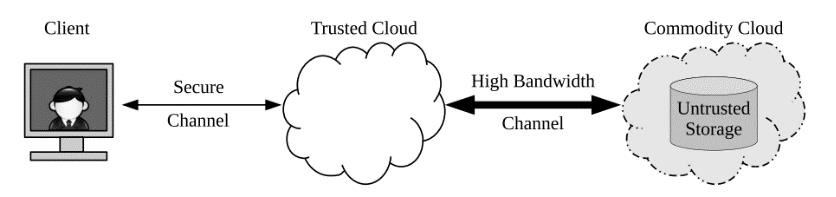
\includegraphics[scale=0.6]{fi4}
\caption{معماری پیشنهادی در 
\cite{4}}\label{fig4}
\end{figure}
هماهنگی بین این دو ابر می‌تواند یکی از مسائل مهم باشد که به‌دقت و ریزه‌کاری نیاز دارد. پس‌ازآن تبادل اطلاعات بین این دو ابر زمان‌بر خواهد بود؛ بنابراین با تغییر درروند ورودی و خروجی و سیاست‌های هر یک از این دو ابر باعث اجبار در تغییر ابر دیگر می‌شود تا همچنان این دو ابر هماهنگ کار کنند؛ اما اگر سیستم به‌خوبی پیاده‌سازی گردد که در عمل بسیار سخت می‌باشد می‌تواند به‌خوبی از منابع اصلی و بسیار حیاتی سیستم محافظت نماید چراکه کاربر هیچ‌گاه به‌طور مستقیم با منابع در تماس نخواهد بود و همین باعث می‌شود تا هکرها نتوانند به‌راحتی حمله خود را طراحی نمایند.
\section{تشخیص نفوذ در سیستم با استفاده از منطق فازی}
توجه به افزایش حملات اینترنتی، ایجاد یک سیستم تشخیص نفوذ برای امنیت سیستم‌ها به یک امر ضروری تبدیل‌شده است. در بیشتر سیستم‌های تشخیص نفوذ ارائه‌شده یک دیتابیس برای ذخیره الگوهای مربوط به حملات وجود دارد که با کمک آن مراقبت از سیستم انجام می‌گیرد. درروش 
\lr{FC-ANN} 
ارائه‌شده 
\cite{7} 
الگوها به‌صورت خودکار یافت می‌شوند و این الگوها در دیتابیس‌های سیستم تشخیص نفوذ ذخیره و مورداستفاده قرار می‌گیرد.

روش پیشنهادی مبتنی بر سه ماژول زیر می‌باشد:
\begin{enumerate}
\item
مشاهده و صف کردن: این ماژول بسته‌های داده‌ای را دریافت می‌کند. سپس داده‌ها را به‌صف مشترک ماژول آنالیز می‌سپارد.
\item
آنالیز و پردازش
\item
گزارش
\end{enumerate}	
کنترل صف به‌صورت چند نخی انجام می‌گیرد. سپس در این صف بسته‌ها موردبررسی قرار می‌گیرند و هشدارهای لازمه تولید می‌گردد.

 هدف این پژوهش 
 \cite{7} 
 طراحی و تحلیل انواع مختلفی از سیستم‌های فازی است که برای تشخیص نفوذ می‌تواند مورداستفاده قرار بگیرد. درنهایت نیز مقاله یک معماری برای کنار هم قرار دادن طبقه بندها ارائه کرده است
 
روش یادگیری قوانین با تکرار

مراحل پردازشی روش به شرح زیر است:
\begin{itemize}
\item[$\bullet$]
تولید یک جمعیت اولیه فازی از قوانین 
\lr{if-then}
\item[$\bullet$]
تولید قوانین جدید فازی 
\lr{if-then} 
به‌وسیله عملیات فازی\/سازی
\item[$\bullet$]
جانشین کردن بخشی از جمعیت موجود با قوانین جدید
\item[$\bullet$]
افزودن دوباره جمعیت
\item[$\bullet$]
اگر شرایط توقف ملاقت شده پردازش را متوقف کن در غیر این صورت به مرحله 
$2$
برو
\end{itemize}
در این سیستم از روش تسریع شده نیز بهره برده شده است. انقدر مراحل یادگیری در این چرخه تکرار می‌گردد تا به نتایج موردنظر برسیم. قوانین فازی در این روش در هر فاز اضافه می‌شوند تا دقت دریافتن جواب افزایش یابد. بخش تسریع دهنده روش ارائه‌شده وزن مثال‌های آموزشی که به‌درستی طبقه‌بندی‌شده‌اند را کاهش می‌دهد تا پردازش چندباره بر روی بخشی از داده‌ها صورت نگیرد.
\section{تشخیص سلسله مراتبی نفوذ به روش ناهنجاری بوسیله شبکه های عصبی}
همراه با رشد سریع شبکه‌های کامپیوتری در طی چند سال اخیر، امنیت در سیستم‌های کامپیوتری مدرن به‌صورت موضوعی بسیار حیاتی و مهم درآمدهاست. در طی دو دهه اخیر تلاش‌های تحقیقاتی فراوانی در زمینه امنیت شبکه صورت گرفته و تکنیک‌های مختلفی برای ساختن شبکه‌های امن ارائه‌شده‌اند. تکنیک‌هایی نظیر فایروال، کنترل دستیابی و تشخیص نفوذ از این قبیل هستند. تمرکز پژوهش انجام‌شده در
\cite{27} 
بر روی تشخیص نفوذ و طراحی و پیاده‌سازی یک سیستم تشخیص نفوذ می‌باشد. سیستم‌های تشخیص نفوذ از دو رویکرد برای تشخیص حملات استفاده می‌کنند: تشخیص ناهنجاری و تشخیص سوءاستفاده. سیستم‌های تشخیص ناهنجاری نفوذ را بر اساس رفتار ناهنجار کاربران یا پردازه‌ها تشخیص می‌دهند، درحالی‌که سیستم‌های تشخیص سوءاستفاده نفوذ را بر اساس الگوهای تعریف‌شده از حملات کشف می‌کنند. سیستم‌های تشخیص سوءاستفاده, تشخیص حملات را تضمین می‌کنند اما برخلاف سیستم‌های تشخیص ناهنجاری قادر به شناسایی حملات جدید یا ناشناخته نیستند. ازلحاظ منبع اطلاعات نیز می‌توان سیستم‌های تشخیص نفوذ را به دودسته سیستم های مبتنی بر میزبان و سیستم‌های مبتنی بر شبکه دسته‌بندی کرد. سیستم‌های مبتنی بر میزبان بر روی اطلاعات جمع‌آوری‌شده در داخل یک سیستم کامپیوتری مجزا عمل می‌کنند، در حالیکه سیستم‌های مبتنی بر شبکه بر ترافیک شبکه نظارت می‌کنند. در این پژوهش یک سیستم تشخیص نفوذ سلسله مراتبی طراحی و پیاده‌سازی شده است که قادر است حملات مبتنی بر شبکه را با روش تشخیص ناهنجاری و به‌وسیله شبکه‌های عصبی تشخیص دهد. شبکه‌های عصبی به دلیل دارا بودن توانایی دسته‌بندی بالا و قدرت تعمیم می‌توانند در سیستم‌های تشخیص نفوذ به‌کاربرده شوند. شبکه نمونه از سه سطح سلسله‌مراتب استفاده می‌کند که هر سیستم تشخیص نفوذ در سطح پایین، گزارشی را به سیستم تشخیص نفوذ در سطح بالا ارسال می‌کند. این سیستم تشخیص نفوذ با دریافت بسته‌ها از شبکه، ویژگی‌های اتصالات شبکه را استخراج کرده و پس از پیش‌پردازش آماری بر روی اتصالات با استفاده از دسته‌بندی شبکه‌های عصبی رفتارهای غیرعادی را در سطح شبکه تشخیص می‌دهد. سیستم تشخیص نفوذ پیاده‌سازی شده از شبکه‌های عصبی در ساختار خود به‌عنوان دسته‌بندی کننده استفاده می‌کند که سیستم‌های تشخیص نفوذ سلسله مراتبی و توزیع‌شده کنونی فاقد چنین ویژگی هستند. شبکه‌های عصبی مورداستفاده شده 
\lr{PBH}
و 
\lr{BP} 
می‌باشند که شبکه عصبی 
\lr{PBH} 
تاکنون در یک محیط واقعی مورد آزمایش قرار نگرفته است و الگوریتم یادگیری شبکه 
\lr{PBH} 
درطی پیاده‌سازی سیستم تشخیص نفوذ پیشنهادی استخراج‌شده است. هدف این پژوهش 
\cite{27}
بررسی و مقایسه کارایی و هزینه دو شبکه عصبی 
\lr{BP} 
و 
\lr{PBH} 
برای تشخیص نفوذ در محیطی عملی و واقعی می‌باشد. نتایج تست شبکه‌های عصبی 
\lr{BP} 
و 
\lr{PBH} 
نشان داد که شبکه 
\lr{PBH} 
با داشتن تعداد نورون‌های مخفی کمتر دارای نرخ اعلان خطای پایین‌تری می‌باشد و درنتیجه کارایی بالاتری نسبت به شبکه 
\lr{BP} 
دارد و همچنین با کاهش تعداد نورون‌های مخفی در شبکه 
\lr{PBH} 
هزینه محاسبات نیز در این شبکه کاهش می‌یابد. 

 
 
 
%%%%%%%%%%%
\begin{thebibliography}{99}
\begin{LTRbibitems}
\resetlatinfont
\bibitem{1}
Rasheed, Hassan. "Data and infrastructure security auditing in cloud computing environments". International Journal of Information Management 34.3 (2014): 364-368.
\bibitem{2}
Bose, Ranjit, Xin Luo, and Yuan Liu. "The Roles of Security and Trust: Comparing Cloud Computing and Banking". Procedia-Social and Behavioral Sciences 73 (2013): 30-34.
\bibitem{3}
Kshetri, Nir. "Privacy and security issues in cloud computing: The role of institutions and institutional evolution". Telecommunications Policy 37.4 (2013): 372-386.
\bibitem{4}
Sood, Sandeep K. "A combined approach to ensure data security in cloud computing". Journal of Network and Computer Applications 35.6 (2012): 1831-1838.
\bibitem{5}
Zissis, Dimitrios, and Dimitrios Lekkas. "Addressing cloud computing security issues". Future Generation Computer Systems 28.3 (2012): 583-592.
\bibitem{6}
Che, Jianhua, et al. "Study on the security models and strategies of cloud computing". Procedia Engineering 23 (2011): 586-593.
\bibitem{7}
A. H. Sung, S. Mukkamala. " Feature Selection for Intrusion Detection using
Neural Networks and Support Vector Machines." Future Generation Computer Systems 32 (2014): 27-40.
\bibitem{8}
Shin, Dong-Hee. "User centric cloud service model in public sectors: policy implications of cloud services". Government Information Quarterly 30.2 (2013): 194-203.
\bibitem{9}
Rong Chunming, Nguyen Son T. Cloud trends and security challenges. In: Proceedings of the 3rd international workshop on security and computernetworks (IWSCN 2011); 2011.
\bibitem{10}
Zhao Gansen, Rong Chunming, Li Jin, Zhang Feng, Tang Yong. Trusted data sharing over untrusted cloud storage providers. In: Proceedings of the 2nd IEEE international conference on cloud computing technology and science (CloudCom 2010); 2010.
\bibitem{11}
Pearson Siani. Toward accountability in the cloud. EEE Internet Comput 2011; 15(4): 64–9.
\bibitem{12}
[12]	Brian Hayes. `Cloud computing'. In: Commun. ACM 51.7 (2008).
\bibitem{13}
Tim Mather, Subra Kumaraswamy and Shahed Latif. Cloud Security and Privacy: An Enterprise Perspective on Risk and Compliance. Editor Mike Loukides. O'Reilly, 2009.
\bibitem{14}
Graham Kirby, Alan Dearle et al. An Approach to Ad hoc Cloud Computing. Tech. rep. St Andrews Cloud Computing Initiative, School of Computer Science, University of St Andrews, Feb. 2009.
\bibitem{15}
Cloud Computing: Bene ts, risks and recommendations for information security. Tech. rep. European Network and Information Security Agency (ENISA), 2009.
\bibitem{16}
Dan Hubbard, Michael Sutton et al. Top Threats to Cloud Computing v1.0. Tech. rep. v1.0. Cloud Security Alliance, Mar. 2010.
\bibitem{17}
Meiko Jensen, Nils Gruschka and Norbert Luttenberger. `The Impact of Flooding Attacks on Network-based Services'. In: ARES '08: Proceedings of the 2008 Third International Conference on Availability, Reliability and Security. Washington, DC, USA: IEEE Computer Society, 2008, pp. 509-513.
\bibitem{18}
Ken Birman, Gregory Chockler and Robbert van Renesse. `Toward a cloud computing research agenda'. In: SIGACT News 40.2 (2009), pp. 68-80.
\bibitem{19}
The Cross-Site Request Forgery (CSRF/XSRF) FAQ. English. CGI Security. Apr. 2010.
\bibitem{20}
[XSS02] The Cross-Site Scripting (XSS) FAQ. English. CGI Security. May 2002.
\bibitem{21}
H. Güneş Kayacık, A. Nur Zincir-Heywood, Malcolm I. Heywood,” Selecting Features for Intrusion Detection: A Feature Relevance Analysis on KDD 99 Intrusion Detection Datasets”, Dalhousie University, Faculty of Computer Science, 6050 University Avenue, Halifax, Nova Scotia. B3H 1W5.
\bibitem{22}
B.B.Sujitha and R.R. Ramani, “Intrusion Detection System using Fuzzy Genetic Approach”, International Journal of Advanced Research in Computer and Communication Engineering Vol. 1, Issue 10, December 2012.
\bibitem{23}
M. Sadiq and Ali Khan,”Rule based Network Intrusion Detection using Genetic Algorithm”, International Journal of Computer Applications (0975 – 8887) Volume 18– No.8, March 2011.
\bibitem{24}
 J.R. Winkler, Securing the Cloud: Cloud Computer Security Techniques and Tactics, Technical EditorBill Meine, Elsevier Publishing, 2011.
 \bibitem{25}
Y. Jadeja and K. Modi, "Cloud computing - concepts, architecture and challenges", in Computing, Electronics and Electrical Technologies(ICCEET), 2012 International Conference on, 2012, pp. 877-880.
\bibitem{26}
A. Soule, K. Salamatian, and N. Taft, "Combining filtering and statistical methods for anomaly detection", in Proceedings of the 5th ACM SIGCOMM conference on Internet Measurement, pp. 31-31, 2005.
\bibitem{27}
A. Kannan, G. Q. Maguire, "Genetic Algorithm based Feature Selection Algorithm for Effective Intrusion Detection in Cloud Networks", 2012 IEEE 12th International Conference on Data Mining Workshops, 2012.
\bibitem{28}
Y. Li, J. Xia, S. Zhang, J. Yan, X. Ai, K. Dai, "An efficient intrusion detection system based on support vector machines and gradually feature removal method", in Expert Systems with Applications 39 (2012) 424–430, 2012.
\bibitem{29}
J.-H. Lee, M.-W. Park, J.-H. Eom, and T.-M. Chung, "Multi-level Intrusion detection system and log management in cloud computing", in Advanced Communication Technology (ICACT), 2011 13th International Conference on, pp. 552-555, 2011.
\bibitem{30}
C. Mazzariello, R. Bifulco, and R. Canonico, "Integrating a network ids into an open source cloud computing environment", in Information Assurance and Security (IAS), 2010 Sixth International Conference on, pp. 265-270, 2010.
\end{LTRbibitems}
\end{thebibliography}
\newpage
\begin{latin}
\section*{ABSTRACT}
\thispagestyle{empty}
Cloud computing model to provide easy access, distributed and pervasive computing resources and shared collective configurable deals. In cloud-based IT capabilities as services that do not require detailed knowledge of infrastructure technologies and have minimal management effort, is provided. Due to this, one of the important issues is the focus of security challenges on modern technology. The most useful aspect of the cloud include: quick and easy implementation model, payments to the amount of use and reduce costs within organizations.Other topics that will be presented by cloud computing paradigm to pay. To evaluate the proposed approach and comparisons with some of the approaches taken in this field assessments indicate that the proposed method is accurate.\\[0.5cm]
\textbf{Key words:}
Cloud Computing, Data Security Improvement, Artificial Neural Networks, Decision Tree
\end{latin}
\end{document}
